\chapter{Distributed representations of automotive scenes}%
\label{chap:a_cognitive_approach_to_represent_automotive_scenes}

In chapter~\ref{chap:research_context} and especially in section~\ref{subsec:knowledge_representation}, we have seen that, already today, there is a plethora of \acfp{ADAS} in intelligent vehicles. 
In future vehicles, the number of modules tackling different sub-tasks necessary to enable (semi-) autonomous driving and to interact with humans inside and outside the car will increase even more.
Given the complexity of the physical world and the recent success of \acp{DNN} in diverse applications, a substantial amount of such modules could be data-driven with increasingly large neural networks under the surface.
In a worst case scenario, each of these systems will encapsulate its own representation of knowledge about the data it processes in complete separation from other, potentially related, systems.
Typically, the representations used rely completely on numerical values and lack possibilities to be enriched or combined with symbol-like representations.
On the other hand, increasingly deep neural network architectures are not only hungry for data to generalize sufficiently beyond the examples they have been trained on, but also tend to require a substantial amount of computational resources.
Although this aspect is more severe for the training process, it becomes more important for mobile applications such as automated vehicles during the deployment phase.

In this thesis, we propose a novel representation for automotive scenes based on modern cognitive modeling techniques, namely the \ac{SPA}.
The \ac{SPA} is one particular example from a family of cognitive architectures commonly referred to as \acp{VSA} (see section~\ref{subsec:vector_based_approaches} and chapter~\ref{chap:introduction_to_vsas} for further details).
One of the key components of these cognitive architectures is to use high-dimensional vectors for representation.
This representational approach offers several desirable features.
High-dimensional vectors are one variant of distributed representations in the sense that information is captured over all dimensions of the vector instead of one single number.
This aspect makes distributed representations more robust to noise in the sense that a few noisy entries influence the overall information carried by the vector less compared to low-dimensional representations.
Furthermore, vector representations allow to encode both, symbol-like and numerical structures in a similar and unified way.
Additionally, the algebraic operations enable manipulation and combination of represented entities into structured representations.
One potential advantage of this approach is that the number of dimensions remains fixed independent of the number of entities combined through the architecture's algebraic operations.
Finally, vectors are a suitable representational substrate to be used in combination with neural networks.
On the one hand, vectors are a natural input to classic \acp{ANN}, but they also offer the possibility to be efficiently implemented in \acp{SNN} using the principles of the \ac{NEF} \parencite[see][but also section~\ref{subsec:implementation_in_snns}]{Eliasmith2013}.
Given a widespread implementation of the representations proposed here in combination with \acp{SNN} as algorithmic substrate within intelligent vehicles, the latter offers the potential to deploy such neural representations on dedicated neuromorphic hardware (cf.\ section~\ref{sec:neuromorphic_HW}).
Although neuromorphic computing hardware as well as the corresponding neural algorithms are mainly used in academic research and often lack the technical maturity required by industrial applications, they show promise to be an energy-efficient option for future automated vehicles once reaching the required level of maturity.

\begin{figure}[t]
    \centering
    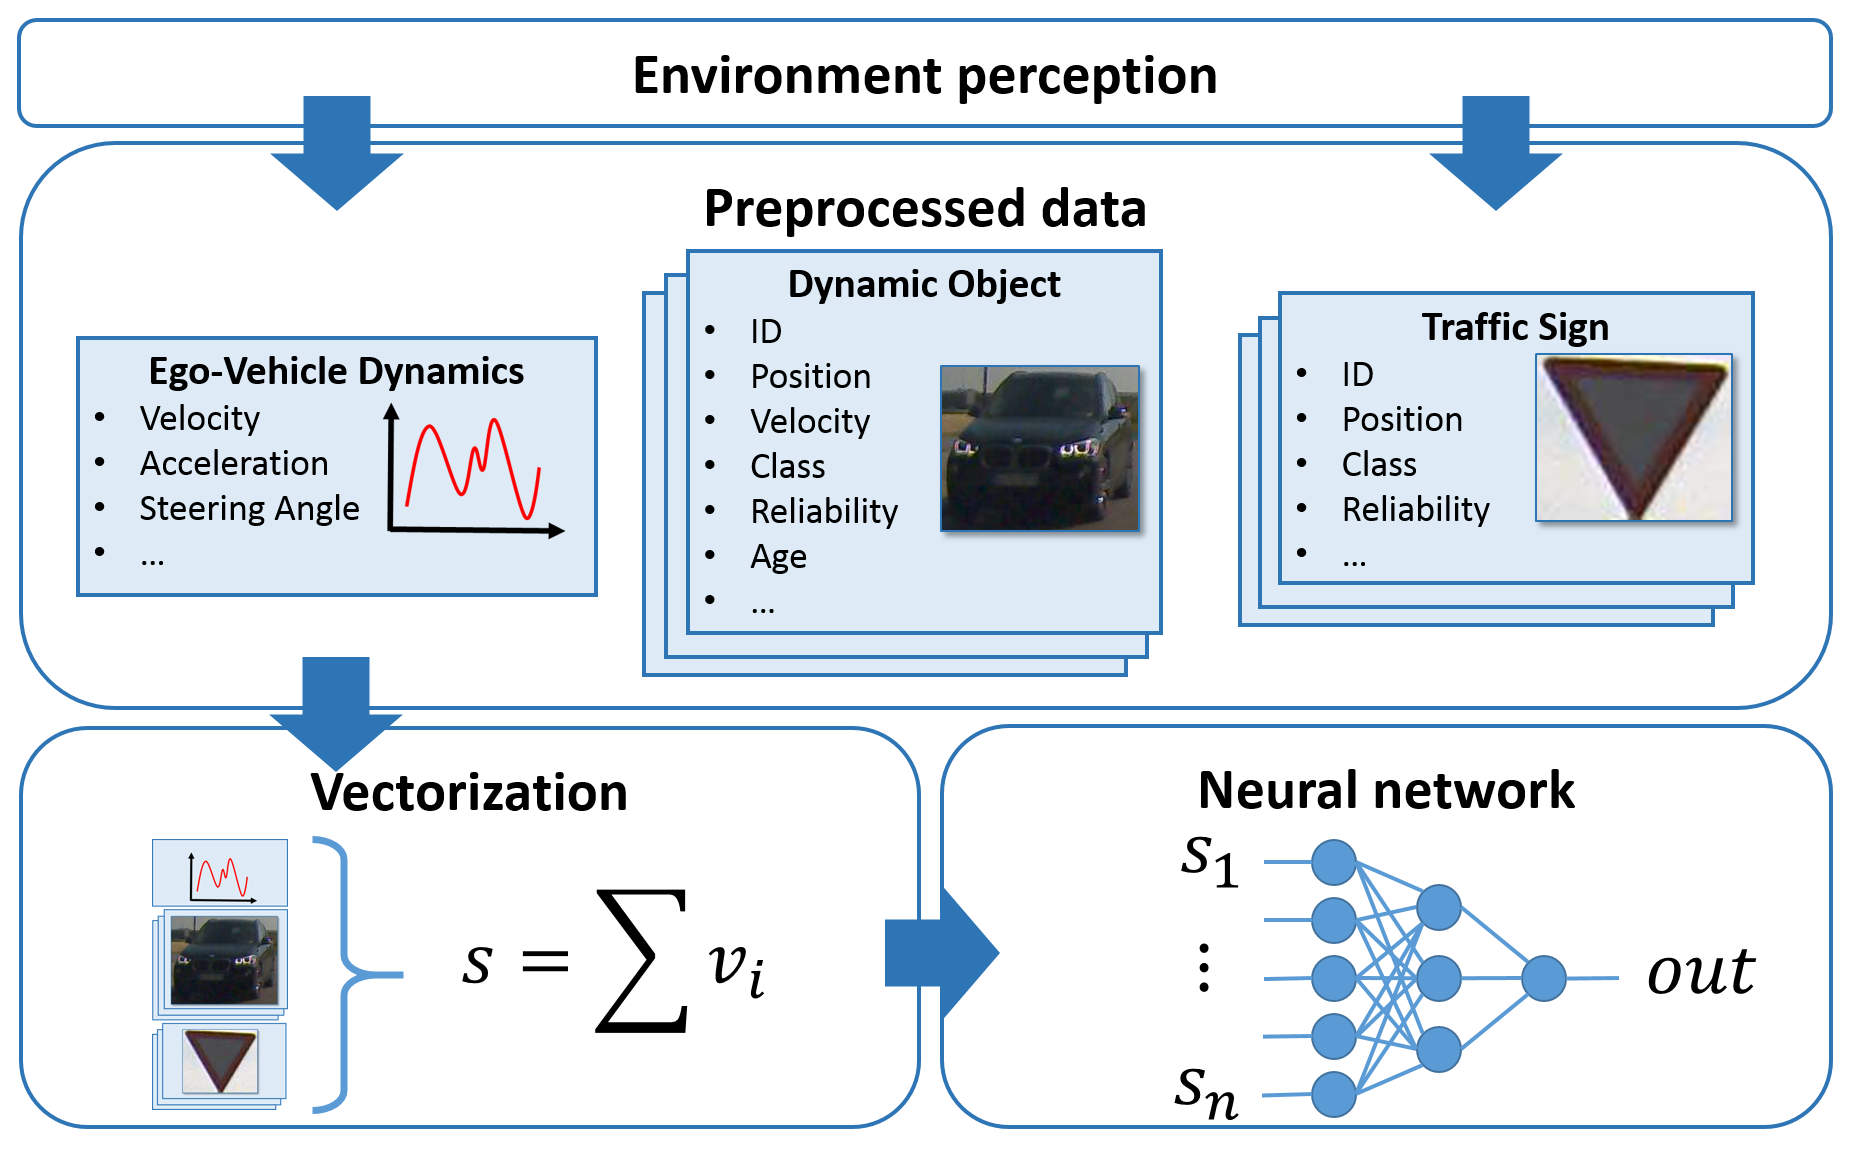
\includegraphics[width=0.8\linewidth]{imgs/system_overview_horizontal.eps}
    \caption{Visualization of the general flow of information of our proposed approach.}
    \label{fig:vectorization}
\end{figure}

In this chapter, we introduce our proposed approach to encapsulate high-level information about automotive scenes in high-dimensional, semantic vectors using the \ac{SPA} as representational substrate.
For this encoding phase, we follow the first two stages, namely \emph{preprocessing} and \emph{representation generation}, of the three-stages process established in \textcite{Gallant2013}.
The third and final stage, \emph{output computation}, will be the subject of subsequent chapters, where we investigate concrete applications and use cases.
The preprocessing stage is the step of creating a suitable vector vocabulary, whereas the representation generation stage is the process of building up structured representations from the atomic vectors within the vocabulary.
Furthermore, we analyze how different types of data could be encoded in such a representation, we show possible variations of how to encapsulate data in vectors and how they influence the final representation.
We also investigate potential limitations imposed by such representations to provide insights into how many concepts can be efficiently encoded in our representations without loss of information.  


\section{Preprocessing stage - generating a vocabulary}%
\label{sec:preprocessing_stage_generating_a_vocabulary}

Figure~\ref{fig:vectorization} visualizes the general flow of information of our proposed system.
To represent high-level information about a scene in an abstract vector representation, we work with already processed data, which comes either from individual sensors performing their own low-level processing, or from a higher-level, central module already fusing information from several sensors.
We simply refer to this step as \emph{environment perception} in Fig.~\ref{fig:vectorization}, whereas its output is referred to as \emph{preprocessed data}.
This data is typically available as lists of objects present in the current scene and is translated into a semantic vector representation by first assigning atomic vectors to entities of interest and then building up more complex, structured representations by using the \ac{SPA}'s algebraic operations.
In this section, we will investigate the first step of assigning atomic vectors to entities of interest, i.e., creating a suitable vector vocabulary.
We have already seen in section~\ref{subsec:vocabs} that such vocabularies can be created in several different ways, which we will here investigate with the specific focus of encoding automotive scenes.

\subsection{What types of data to encode?}%
\label{subsec:what_types_of_data_to_encode_}

The data to be encoded in a semantic vector substrate depends not only on the information available from the current sensor-setup, but also on the task at hand.
For instance, if we want to classify the current driving context (like in chapter~\ref{chap:driving_context_classification}), the relevant information might be different to the task of predicting a vehicle's trajectory (like in chapter~\ref{chap:behav_pred}).
Here, we give an overview of what information in general is available in an intelligent vehicle and how to encode it in a semantic vector substrate.
We distinguish between symbol-like information such as the type of a dynamic object or numerical information such as the current acceleration of the ego-vehicle.
In this section, we focus mainly on the symbol-like information, which is suitable to be represented using a single atomic vector or an algebraic combination of several atomic vectors.
In section~\ref{subsec:different_vector_representations_for_numerical_values}, we will focus on numerical information and different options of encoding them in vectors.
Here, we will closely follow the structure of section~\ref{sec:cognitive_modelling_with_vsa} and present different possibilities to generate a vocabulary of atomic vectors to built structured representations upon.

If the vectors in the vocabulary are not chosen at random, the general goal when creating the vocabulary is to generate atomic vectors that carry inherent structure or meaning.
This meaning is typically reflected by similar concepts being mapped to similar vectors.
However, there are several possible notions of similarity that can be encoded in the vocabulary, which we will specify in this section.

\subsubsection{Visual similarity}%
\label{ssubsec:visual_similarity}

A first simple and comprehensible notion of similarity is visual similarity between two entities: \enquote{do they look similar}. 
Encoding this notion in vectors, we would expect the vector representations to encapsulate this type of similarity within the relation between the vectors, meaning that vectors representing visually similar entities will have large cosine similarity.
In conjunction with other information, this type of similarity could be useful to detect a wrong classification, in case it has high similarity to another one that makes more sense in the situation or context at hand.
An example would be the German traffic signs indicating a speed limit of \SI[per-mode=symbol]{30}{\kilo\meter\per\hour} and \SI[per-mode=symbol]{80}{\kilo\meter\per\hour}, which are both circular with a red frame and a similar looking black number on white background in the middle.
However, encountering a speed limit sign of \SI[per-mode=symbol]{30}{\kilo\meter\per\hour} in an urban situation is more plausible than a sign indicating a speed limit of \SI[per-mode=symbol]{80}{\kilo\meter\per\hour}.

\subsubsection{Similarity of motion}%
\label{ssubsec:similarity_of_motion}

Another notion of similarity, that is a candidate to be encoded in a vector vocabulary, is the similarity of motion properties.
For instance, bicycles and motorcycles have more similar motion properties (dynamics of vehicles with two wheels) than for example a pedestrian and a truck.
Apart from motion properties such as dynamics of the movement, the number of wheels or the mean expected velocity the direction of movement of traffic participants can be a notion of similarity to be encoded in the vocabulary.
For instance, traffic participants such as bicycles or cars moving towards us might be encoded more similarly to each other than to parked cars or those moving away.
Furthermore, some entities are more likely to change their motion or direction: while traffic lights frequently alternate and parked cars might start moving, trees, buildings and traffic signs are expected to remain static. 
The notion of similarity of motion can be useful in various ways.
In a first step, knowing the motion of other traffic participants could help in classifying the situation: on a multi-lane highway we would expect cars around us to move in the same direction, whereas in an urban driving situation, the motion of other traffic participants is more diverse. 
Additionally, this notion of similarity could potentially help in focusing the system's attention or, more precisely, use computing power more efficiently on entities that are more relevant to decision making.
For example, a change of the \enquote{motion status} (e.g., when a bus stops) might need particular attention.

\subsubsection{Semantic similarity}%
\label{ssubsec:semantic_similarity}

While visual similarity already captures a significant part of perceivable information about entities in automotive context, there is further information, that could be encoded in the vector vocabulary and that is different, or maybe even contrary to visual similarity. 
Considering automotive situations, we as humans do not only assess them based on visual appearance but also by incorporating underlying and, most likely, previously acquired knowledge about the objects in the scene.
This underlying information can be considered the semantic aspect.
Revisiting the aforementioned example, the speed limit sign for \SI[per-mode=symbol]{30}{\kilo\meter\per\hour} is \emph{visually} more similar to \SI[per-mode=symbol]{80}{\kilo\meter\per\hour} than to \SI[per-mode=symbol]{20}{\kilo\meter\per\hour}.
However, in the context (or semantics) of an automotive situation such as driving in an urban environment, speed limit signs for \num{20} and \SI[per-mode=symbol]{30}{\kilo\meter\per\hour} should be contextually or semantically more similar to each other than signs for \num{30} and \SI[per-mode=symbol]{80}{\kilo\meter\per\hour}, since they are more likely to appear in similar contexts and both describe the traffic rule restricting driving to slow velocities.

Semantic similarity is not quite as intuitive as visual similarity. 
In general, we want to encode objects and concepts sharing similarity in \emph{meaning} in vectors with a high cosine similarity.
However, it is not intuitively clear what similar meaning actually refers to and how to properly define semantic similarity in an automotive context.
In the field of generating word embeddings for natural language processing, the typical assumption is that words sharing similarity in meaning appear in close proximity with high probability within text corpora.
This assumption could be transferred to automotive context as well, for instance, thinking of traffic signs indicating speed limits appearing in similar contexts or driving situations.
For example, traffic signs indicating moderate speed limits are more likely to appear in urban driving situations compared to higher speed limit signs being less likely to appear in such a context.
However, on the one hand, it is not clear how to transfer this approach to other object classes such as traffic participants, whose appearance probability is less context dependent than for traffic signs. 
On the other hand, the process of automatically training a system to learn this form of embedding is not clear as it would probably demand for another learning model to extract contextual information from the rich features of driving contexts.
Therefore, we will now focus on the potential meaning of objects appearing in an automotive environment and how their semantic meaning could be embedded into a vector representation while leaving aside intangible concepts representing vehicle dynamics such as \emph{velocity} or \emph{acceleration}.

\paragraph{Traffic signs}%
\label{par:traffic_signs}

Any traffic sign carries an explicit meaning defined in traffic law and anyone with a driver's license should know its meaning and be able to immediately explain it.
The meaning of a traffic sign is an instruction for the driver's behavior to, for instance, not surpass a certain velocity or to give way to other traffic participants. 
There are sub-groups of signs with similar meanings such as signs indicating speed limits, prescribed direction or warnings for potentially dangerous road conditions or to pay increased attention.
Encoding the semantic structure of traffic signs in a vector vocabulary, we expect not only all traffic signs will be similar but also that all signs within a certain sub-group end up being more similar to one another compared to signs from other subgroups. 
For instance, signs indicating speed limits should be similar to one another, ideally with signs indicating lower velocities such as \SI[per-mode=symbol]{20}{\kilo\meter\per\hour} and \SI[per-mode=symbol]{30}{\kilo\meter\per\hour} should be more similar than \SI[per-mode=symbol]{30}{\kilo\meter\per\hour} and \SI[per-mode=symbol]{130}{\kilo\meter\per\hour}. 
Beside their explicit meaning, the number of traffic signs is finite and limited to a small number compared to the number of words in a typical human-level language vocabulary.
Therefore, it is possible to manually engineer their semantic similarity, which makes it easier to impose our human understanding onto the structure, although the resulting vocabulary will most likely differ from the structure an unsupervised learning model would pick up from the data. 

\paragraph{Traffic participants}%
\label{par:traffic_participants}

While the meaning of traffic signs is clear and explicit, it is far more difficult to derive a meaning of a traffic participant such as a car or a pedestrian or a measure of similarity between them.
It is unclear if a truck is semantically more similar to a motorcycle or to a car without considering any contextual information while ignoring similarity of motion properties, which have already been discussed in section~\ref{ssubsec:similarity_of_motion}.
However, if we do consider contextual information, we as humans decide intuitively if a truck and a motorcycle are more similar when compared to a pedestrian by, e.g., considering their velocity of motion or their vulnerability.
We also know from experience that the meaning of a car approaching from the right potentially means that it has the right of way when we encounter a situation at a crossroads without traffic signs indicating other right of way rules. 
Hence, the situational context has a significant impact on comprehending the \emph{meaning} of traffic participants, which in most cases directly results in appropriate driving actions to take such as decelerating or changing the lane.
However, such a situational understanding is impossible to derive without additional information such as position, velocity or direction of each traffic participant.
Consequently, it is impossible to encapsulate such semantic or contextual similarity in a vector vocabulary directly but rather encode another notion of similarity for atomic vectors of traffic participants and built situational similarity through structured representations using the \ac{VSA}'s algebraic operations.

\subsubsection{Summary on similarity}%
\label{ssubsec:summary_similarity}

All of the aforementioned notions cover a certain aspect of similarity.
Ideally, it is desirable for a vector vocabulary to encapsulate more than one notion of similarity comparable to a human understanding all these different aspects of similarity.
However, it is not clear if it is helpful or even possible, to encapsulate several notions of similarity into one coherent vector vocabulary or if it is more suitable to have separate vocabularies for each similarity of interest and combine them in structured representations using the \ac{VSA}'s algebraic operations as mentioned, e.g., in \textcite{Crawford2016}.
For the remainder of this section, we give an overview over different options of how to generate vector vocabularies encoding their own notion of similarity.

\subsection{Random and manually engineered vocabularies}%
\label{subsec:basic_random_vocabularies}

The simplest possible option to generate a vocabulary of atomic vectors is to sample them randomly, in case of continuous \acp{VSA} such as the \ac{SPA}, from the $D$-dimensional unit sphere \parencite{Voelker2017}.
Naturally, randomly chosen atomic vectors do not carry semantic meaning or any intended notion of similarity.
However, given a sufficiently large dimension $D$ of the chosen \ac{VSA} and its theoretical properties (see chapter~\ref{chap:introduction_to_vsas}), we can assume that randomly chosen vectors will be dissimilar enough to avoid accidentally mistaking them for one another.
Another advantage of this simple approach is that it is comparatively easy to create a vocabulary avoiding any complex learning system to embed the concepts of interest in semantic vectors.
On the other hand, if specific applications demand for the vectors to actually carry semantic information meaning that similar concepts need to be mapped to similar vectors for the application to succeed, this simple approach can be extended by manually engineering a vocabulary reflecting the desired similarity structure.
This is typically achieved by randomly choosing a set of auxiliary vectors and building atomic vectors with the desired similarity from them through the \ac{VSA}'s algebraic operations (cf.\ section~\ref{subsec:vocabs}).
However, this approach is only feasible and appropriate for rather small sized vocabularies since manually designing semantic vectors with certain similarity properties becomes intractable quickly with an increasing number of concepts to be embedded.
Furthermore, manually designing vocabularies involves design choices by human engineers, which is sensitive to potentially undesired biases in the similarity structure of the vectors.
For instance, the example vocabulary created in section~\ref{subsec:vocabs} solely focused on the motion characteristics and typical actuators of different traffic participants.
However as mentioned before, there are many other possible similarity structures such as visual (or auditory), motion or semantic similarity, to be considered when designing the vocabulary.

\subsection{Visual vocabularies}%
\label{subsec:visual_vocabularies}

The next step to generate vocabularies with an inherent similarity structure is to encapsulate visual similarity in a vector embedding.
Visual similarity is an intuitive concept and we can make an educated guess that this notion of similarity could be beneficial for several tasks when encoded directly in the vector vocabulary. 
However, it is preferable to automatically learn to embed visual similarity in vectors instead of manually engineering the similarity between entities as this approach does not scale well for an increasing number of items to be encoded.
One option for such an automated learning system to generate a structured vocabulary encoding visual similarity is to adapt a \acf{DNN} for image classification.
Such a neural network can be thought of as an efficient image compression machine.
While earlier and intermediate layers learn sensibility to visual features such as edges and shapes, the information in the image is compressed into a single dimension, namely the label, at the final classification layer.
Considering the special case of a \acf{CNN}, one option would be to simply use the output of one of the later fully-connected layers and regard it as a vector since we expect the vectors of visually similar images to be similar regarding their cosine similarity.
Here, we focus our efforts of generating a visual vector vocabulary on items of interest to automated driving, namely the aforementioned categories of traffic signs and traffic participants.

\subsubsection{Traffic signs}%
\label{ssubsec:traffic_signs}

\begin{figure}[t]
    \centering
    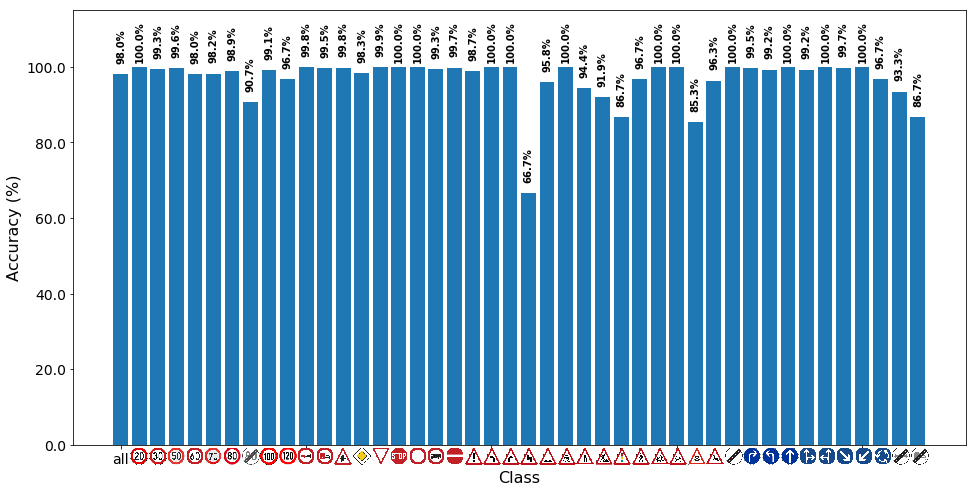
\includegraphics[width=1.\linewidth]{imgs/CNN_GTSRB_performance_plot.eps}
    \caption{Accuracy performance of the \ac{CNN} for traffic sign classification on the test part of the \ac{GTSRB} data set for all traffic signs (most left bar) and all individual traffic signs.}
    \label{fig:CNN_GTSRB_performance_plot}
\end{figure}

To achieve the task of encoding traffic signs encountered by an automated vehicle, we employ a variant of the state-of-the-art \ac{CNN} for traffic sign classification proposed by \textcite{Ciresan2012}.
We train a simplified version of this network on the \acf{GTSRB} \parencite{Stallkamp2012}, which is a data set including a total of \num{51840} images of \num{43} different classes of traffic signs.
Although the \ac{GTSRB} data set does not contain all possible traffic signs, it is a suitable and sufficiently large data set for our purposes of learning a visual vector vocabulary.
The original multi-column network proposed by \textcite{Ciresan2012} combines several variants of the same network architecture trained on the original input images as well as four different, high-contrast normalized versions of the input images by averaging the predictions of all individual networks.
For simplicity, we only use a single-column version of this network to generate a visual vector vocabulary. 
Figure~\ref{fig:CNN_GTSRB_performance_plot} shows the classification accuracy of our network on the test part of the \ac{GTSRB} data set for all traffic signs (most left bar) and all individual signs.
The network achieves competitive results with \SI{98}{\percent} classification accuracy on all traffic signs while detecting all but four traffic signs with accuracy values way above \SI{90}{\percent}, which is sufficient for our purposes.

\begin{figure}[t]
    \centering
    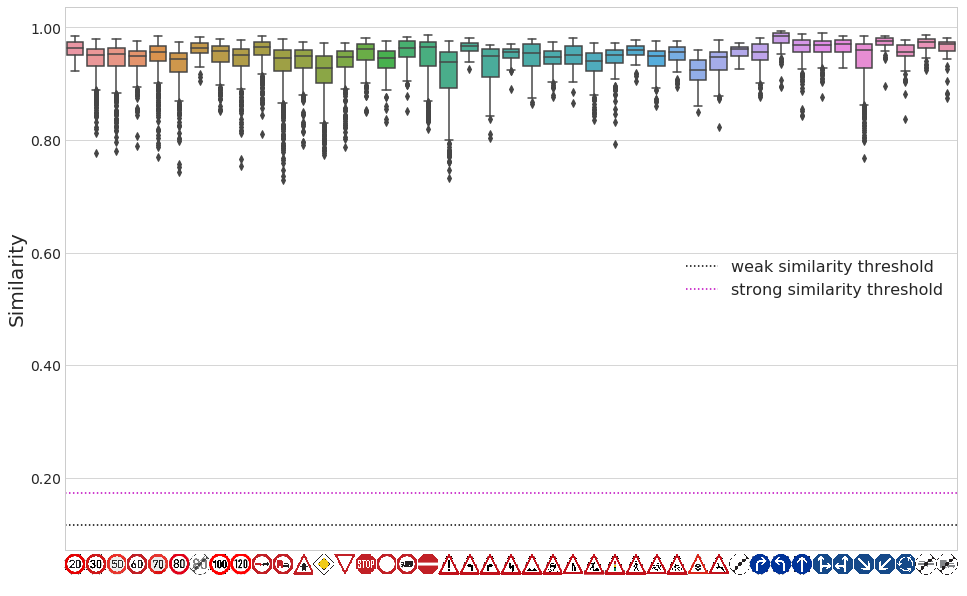
\includegraphics[width=1.0\linewidth]{imgs/Visual_vocab_traffic_signs_similarity_with_representative_vecs.eps}
    \caption{Boxplots depicting the cosine similarities between the representative (mean) vector for each traffic sign class and all individual vector samples it has been created from.}
    \label{fig:visual_vocab_traffic_signs_similarity_with_representative_vecs}
\end{figure}

To generate our vocabulary vectors, we cut off the classification layer with softmax activation and use the previous \num{300}-dimensional, fully connected layer as output.
With this simple adaptation, the \ac{CNN} produces a \num{300}-dimensional vector as output for each image fed into the network. 
To generate a representative vector for each class of traffic signs, several approaches are conceivable, including (weighted) mean and median by dimension or regarding whole vectors.
In this work, we choose the simple mean to create this representative from several examples.
To select the example vectors to calculate the representative mean vector from, we select only instances for which the network produces correct classification predictions alongside high confidence values from the test subset of the \ac{GTSRB} data set.
The great majority of examples even satisfies the restriction of \SI{100}{\percent} confidence, hence we use that strict confidence value to avoid including examples the network is doubtful about, which might deteriorate the properties of the representative vector. 
This procedure leads to a representative vector that \enquote{points} to the center of mass of all (high confidence) vectors of each class of traffic signs.
However, we still need to confirm that these representative vectors fulfill the properties they have been constructed for, namely sharing a high cosine similarity with all individual samples from the respective traffic sign class.
Figure~\ref{fig:visual_vocab_traffic_signs_similarity_with_representative_vecs} shows the cosine similarity between each vocabulary vector encoding each class of traffic signs with all individual vector samples it has been created from.
As expected, we observe high similarity values close to the maximum value of \num{1} and way above both, weak and strong, similarity thresholds for \num{300}-dimensional vectors.

\begin{figure}[t]
    \centering
    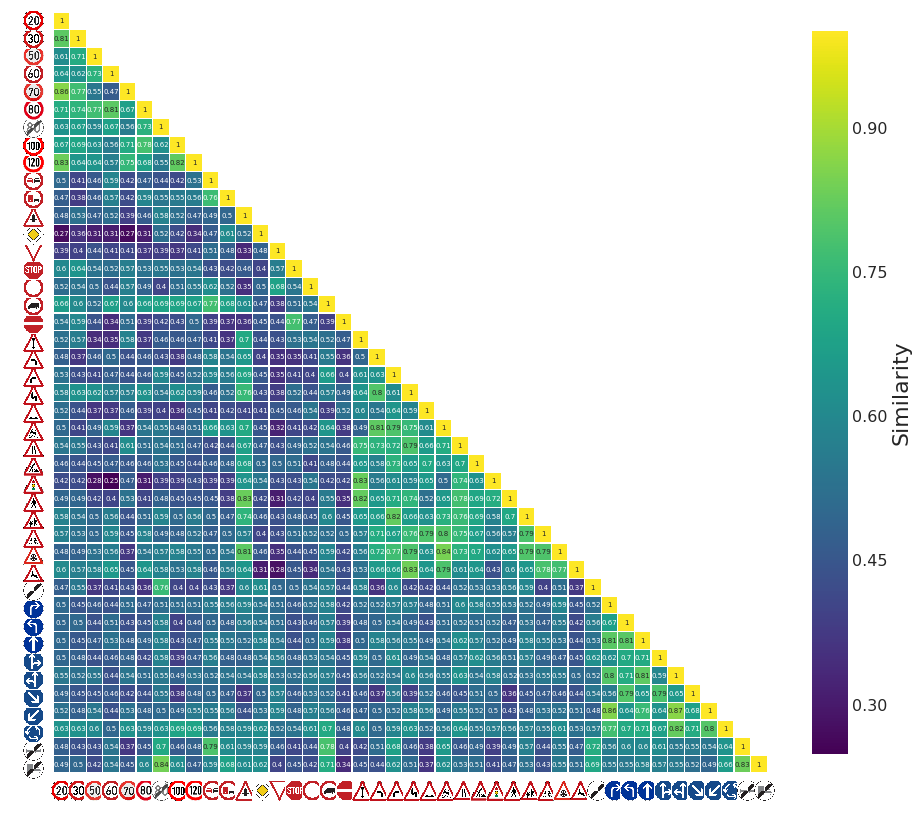
\includegraphics[width=1.0\linewidth]{imgs/visual_vocab_traffic_signs_internal_similarities.eps}
    \caption{Pairwise similarities between representative vectors encoding traffic signs in a visual vector vocabulary.}
    \label{fig:visual_vocab_traffic_signs_internal_similarities}
\end{figure}

Furthermore, we expect these representative vectors, which are now our vocabulary vectors encoding the respective traffic signs, to resemble the visual similarity structure of the image classes. 
To confirm this inherent similarity structure, we calculate pairwise similarities between all vectors in the vocabulary, which are visualized in Fig.~\ref{fig:visual_vocab_traffic_signs_internal_similarities}.
We observe similarities in groups of signs indicated by green areas in the heat map visualization.
Most prominent are the high similarities in three groups of traffic signs forming green triangles in the heat map.
These groups are round signs with red borders (top left corner), triangular warning signs with red borders (middle right) and blue signs indicating driving directions (close to bottom right).
Furthermore, several signs stand out particularly: The traffic sign indicating \enquote{Priority ahead}, which is a red triangle just like any warning signs, indeed shows high similarity to all warning signs.
Similarly, the traffic sign indicating no entry for trucks, a red circle with a black truck inside, looks a lot like speed limit signs and indeed shows a high similarity to all speed limit signs.
Consequently, we conclude that it is possible to encode visual similarity with an automatic learning approach using \acp{CNN} to encapsulate the visual features of a given data set into a vocabulary of semantic vectors.

\subsubsection{Traffic participants}%
\label{ssubsec:traffic_participants}
\begin{center}
	\begin{tabular}{|c|c|c|c|c|c|}
		\hline
		 & BICYCLE & CAR & MOTORCYCLE & PERSON & TRUCK\\ \hline
        Classification accuracy & \SI{94.3}{\percent} & \SI{76}{\percent} & \SI{55}{\percent} & \SI{82.6}{\percent}& \SI{99}{\percent}\\ \hline
	\end{tabular}
	\captionof{table}{Classification accuracy of the adapted VGG19 network for our selected \num{5} classes of traffic participants.}
	\label{tab:traffic_participant_visual_accuracy}
\end{center}

To encode the object categories for traffic participants \emph{Bicycle}, \emph{Car}, \emph{Motorcycle}, \emph{Pedestrian}, \emph{Truck} necessary to properly represent dynamic automotive scenes in visual vectors, we employ an approach similar to the one used for traffic signs.
We adopt a general purpose image data set, the Imagenet data set \parencite{Deng2009}, which includes suitable categories for all of these classes.
As an additional advantage, Imagenet is a widely used data set, so there already exists a number of successful classification networks, which can be adapted for our purposes.
Concretely, we employ the following categories as they appear visually most suitable for the objects categories we want to encode:
We use the original labels 'SAFETY BICYCLE' to learn visual vectors for \emph{Bicycle}, 'USED CAR' for \emph{Car} (other car categories include ambulances and many sports / racing cars), 'MOTORCYCLE', 'PERSON' for \emph{Pedestrian} (since there is no special category for people in the vicinity of roads) and 'TRUCK'.
For each category, there are at least \num{1200} images available in the data set.

\begin{figure}[t]
    \centering
    \resizebox{.95\textwidth}{!}{%
        \subfloat[\label{subfig:visual_vocab_traffic_participants_similarity_with_representative_vecs}]{%
            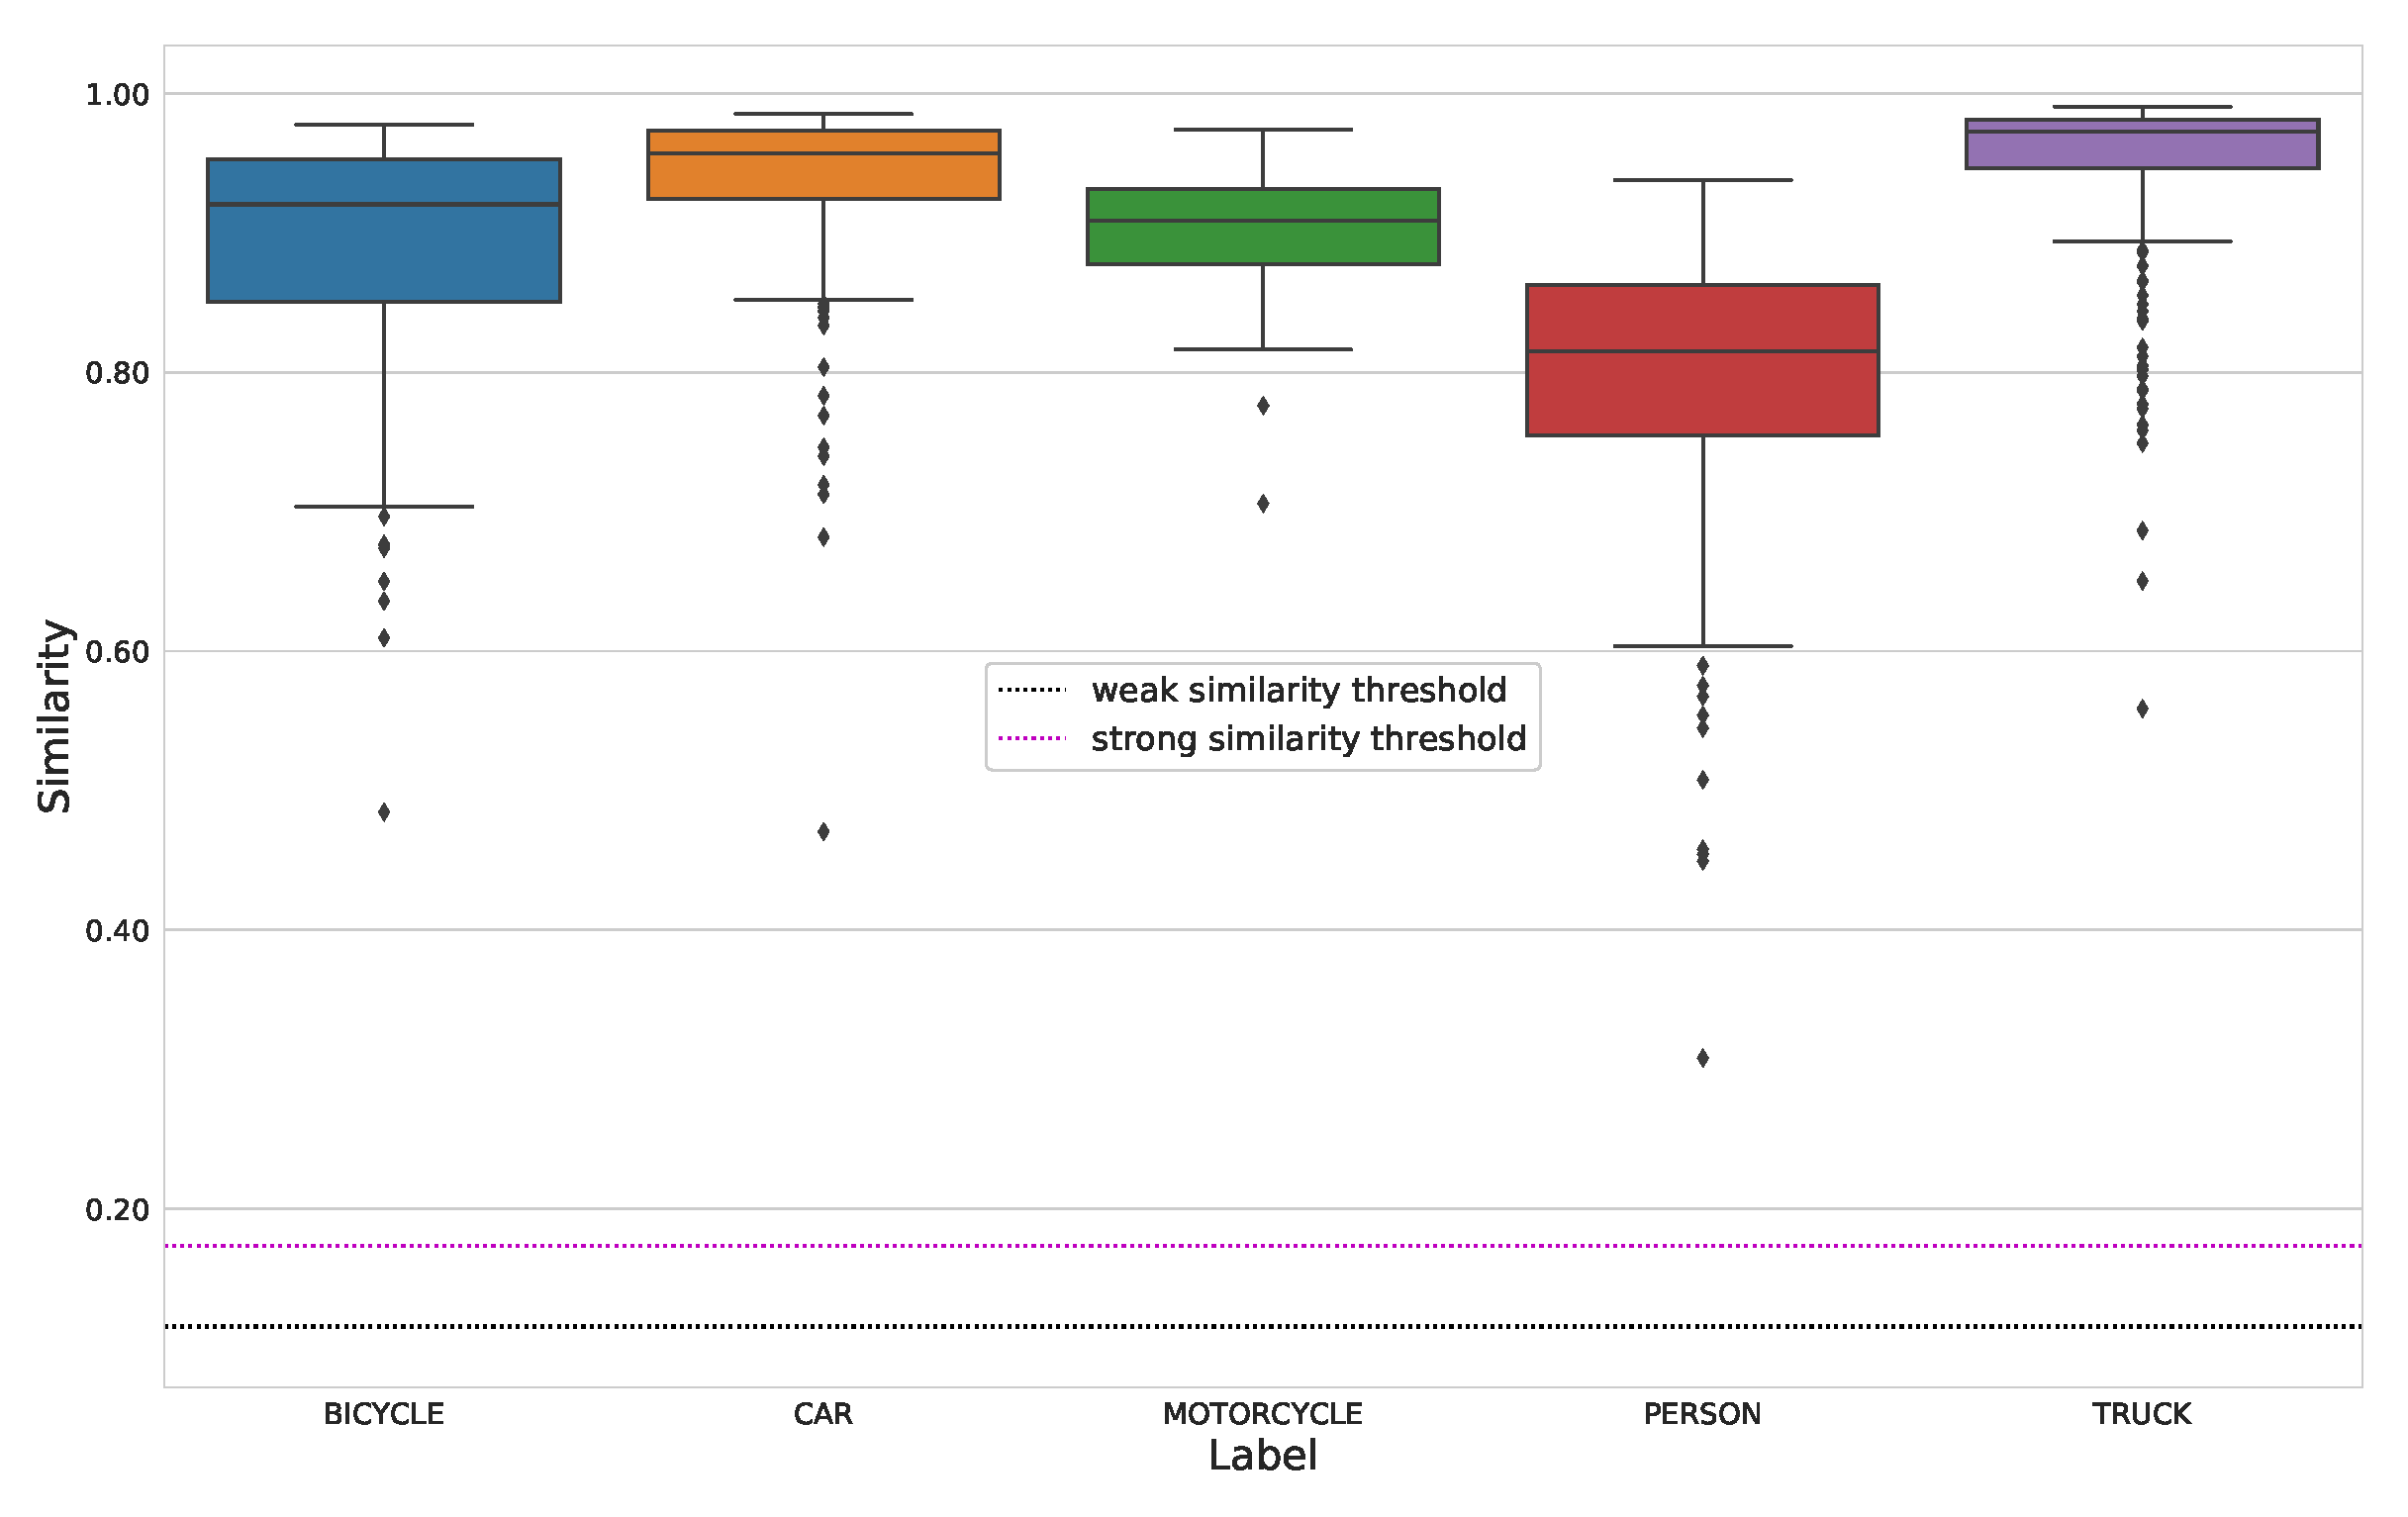
\includegraphics[height=3.5cm]{imgs/Visual_vocab_traffic_participants_similarity_with_representative_vecs.eps}
        }
        \subfloat[\label{subfig:visual_vocab_traffic_participants_internal_similarities}]{%
            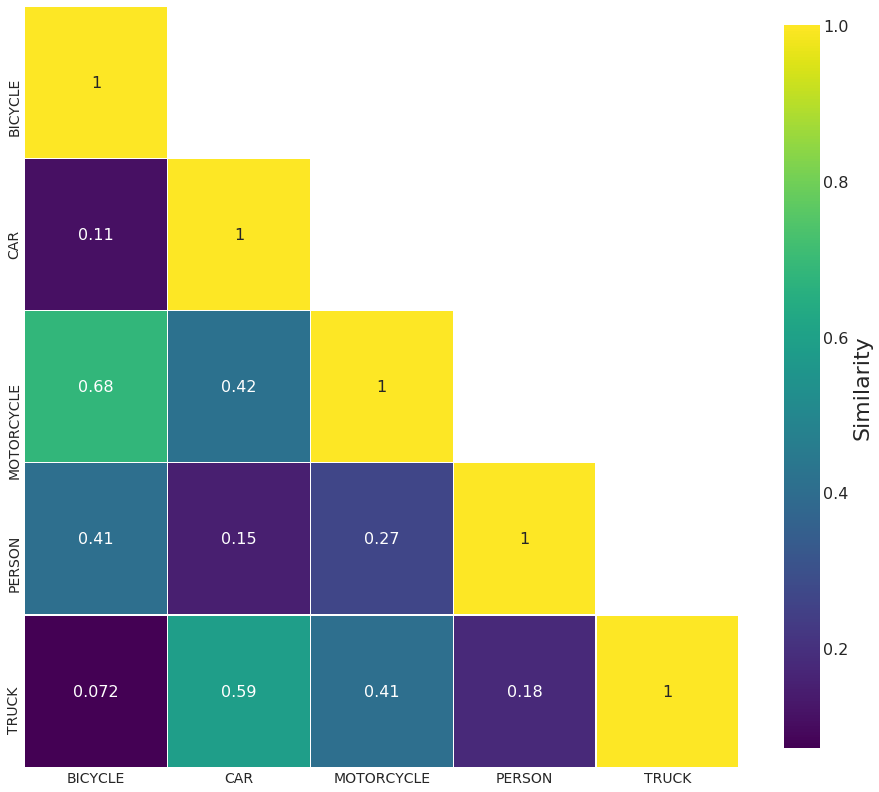
\includegraphics[height=3.5cm]{imgs/visual_vocab_traffic_participants_internal_similarities.eps}
        }
    }
    \caption{Similarity plots for the visual vocabulary vectors representing traffic participants.~\protect\subref{subfig:visual_vocab_traffic_participants_similarity_with_representative_vecs} Boxplots depicting the cosine similarities between the representative (mean) vector for each traffic participant class and all individual vector samples it has been created from.~\protect\subref{subfig:visual_vocab_traffic_participants_internal_similarities} Pairwise similarities between representative
    vectors encoding traffic participants in our visual vector vocabulary.}
    \label{fig:visual_vocab_traffic_participants}
\end{figure}

While there is a number of state-of-the-art classification networks available achieving good results on the Imagenet data set, we are looking for a network with only moderately complex structure for the sake of implementation simplicity and ease of adaptation, while performance is of secondary priority.
VGG19 is a deep \acf{CNN} proposed by \textcite{Simonyan2014} with a decent performance on the Imagenet data set (top 1 performance \SI{73}{\percent} and top 5 performance \SI{91}{\percent}) and a comparatively simple layer by layer architecture that allows easy extraction of results from intermediate layers.
Our goal is to train a variant of the VGG19 network on these \num{5} classes and extract feature vectors of an intermediate layer to use them as vocabulary vectors.
Therefore, we adapt the original network architecture in the following way:
We cut off the last two fully connected layers as well as the classification layer and replace them with a fully connected, \num{300}-dimensional layer and a \num{5} dimensional classification layer. 
We train the modified network using the categorical cross entropy loss and \enquote{standard} stochastic gradient descent optimization.

Table~\ref{tab:traffic_participant_visual_accuracy} depicts the classification performance of our adapted VGG19 network for the \num{5} selected traffic participant categories.
Except for the \enquote{MOTORCYCLE} class, the network achieves decent classification results above \SI{75}{\percent}, which is sufficient for our purposes.
Similar to the creation of the visual vocabulary for traffic signs, we calculate the mean of vectors produced by the second to last of the network's layers when making correct predictions with \SI{100}{\percent} confidence.
Even for the \enquote{MOTORCYCLE} class, there are at least \num{139} of such vectors available, whereas for all other classes, we have at least \num{200} of such vectors.
To confirm that the vocabulary vectors created in this fashion are visually representative enough for each class, we calculate the cosine similarity between the vocabulary vectors and all vector samples they have been created from.
Figure~\ref{subfig:visual_vocab_traffic_participants_similarity_with_representative_vecs} visualizes these similarities as box plots.
Similar to the traffic sign vocabulary, we observe high similarity values close to the maximum value of \num{1} and way above both, weak and strong, similarity thresholds for \num{300}-dimensional vectors.
We also calculated pairwise similarities between all vocabulary vectors encoding traffic participants, which are visualized in Fig.~\ref{subfig:visual_vocab_traffic_participants_internal_similarities}.
As expected, visually similar classes such as \enquote{BICYCLE} and \enquote{MOTORCYCLE} as well as \enquote{CAR} and \enquote{TRUCK} share relatively high cosine similarities.
Less similar, but still significantly higher than the similarity thresholds, are traffic participants sharing the visual features of persons such as \enquote{PERSON} and \enquote{BICYCLE}, \enquote{PERSON} and \enquote{MOTORCYCLE} as well as \enquote{BICYCLE} and \enquote{MOTORCYCLE}.
All other pairs have similarity values in the order of magnitude or below the similarity thresholds and are therefore considered dissimilar while we do not attach the greatest importance to the actual (low) numbers.
Consequently, we can conclude, that we are able to encode visual similarity of traffic signs as well as traffic participants in a visual vector vocabulary.

\subsection{Semantic vocabularies}%
\label{subsec:semantic_vocabularies}

\begin{figure}[t]
    \centering
    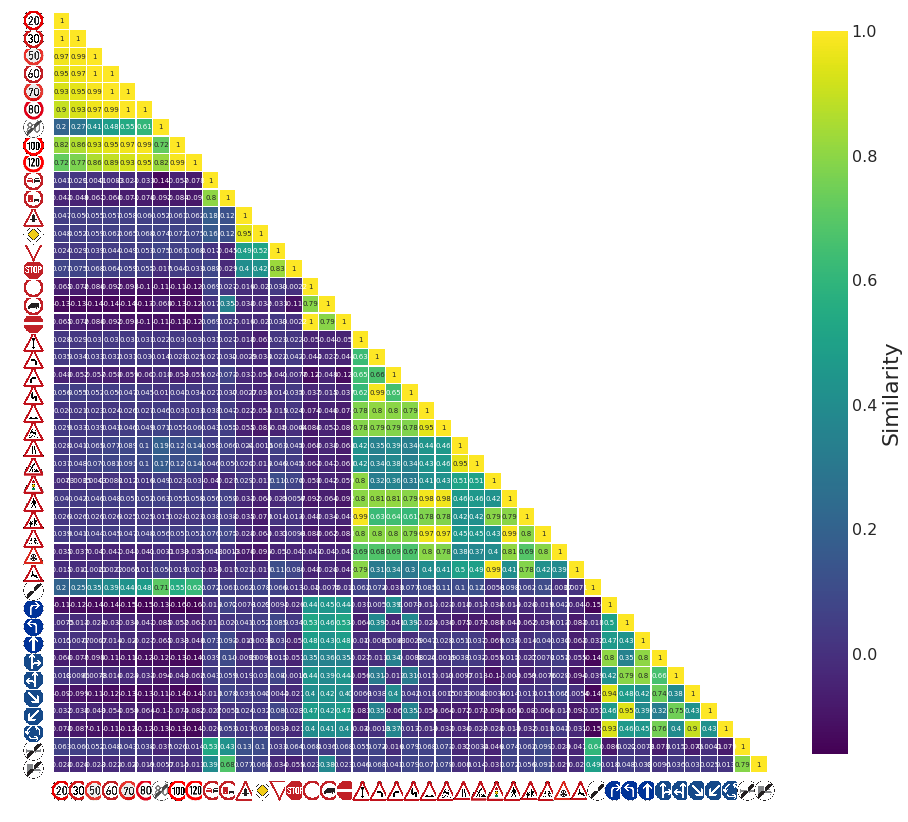
\includegraphics[width=1.\linewidth]{imgs/semantic_vocab_traffic_signs_internal_similarities.eps}
    \caption{Pairwise similarities between representative vectors encoding traffic signs in a manually designed semantic vector vocabulary.}
    \label{fig:semantic_vocab_traffic_signs_internal_similarities}
\end{figure}
In this section, we go one step further and try to encapsulate semantic similarity structures within a vector vocabulary.
As discussed in section~\ref{ssubsec:semantic_similarity}, semantic similarity as a concept is comparatively intuitive for traffic signs and less obvious for other objects, such as traffic participants.
Furthermore, we also highlighted in that section that semantic similarity in other domains such as language modeling typically unfolds through proximity, i.e., that similar words appear in similar contexts or proximity within the text.
While this could give a hint towards what kind of learning procedure could be used to automatically generate a semantic vocabulary in automotive context, availability of suitable data sets is rather limited.
Analogously to the visual vocabulary, we consider the encoding of traffic signs and traffic participants separately in this section as well. 

\subsubsection{Traffic signs}%
\label{ssubsec:traffic_signs}

Our goal is to encode the meaning of traffic signs, i.e., the driving instruction or traffic rule they indicate to the driver in a semantic vector vocabulary.
As with visual similarity, this goal could be achieved by either manually engineering the similarity structure through the \ac{VSA}'s algebraic operations from randomly chosen atomic vectors or through some automated learning approach.
If we were to learn this similarity structure automatically, there are two possible approaches. 
Similar to word embedding algorithms for language, we could either learn the meaning of traffic signs explicitly from a large  corpus of text that describes traffic signs and their meanings in context.
Alternatively, we could try to learn the semantic meaning of traffic signs implicitly from many dynamic driving situations.
Unfortunately, there are no suitable data sets available for either of the aforementioned learning approaches.
Additionally, an implementation of the latter, implicit learning approach would be quite complex, as it would require additional steps to extract structural understanding from the driving scene upon on which the vocabulary generation system needs to be built.
To our knowledge, such a system does not exist.
Consequently, the only remaining option is to manually design the desired similarity structure as described in section~\ref{subsec:basic_random_vocabularies}.

To encode the semantic meaning of traffic signs, we choose atomic vectors for the basic building blocks of the representation at random and create semantic structure by employing the algebraic operations of the \ac{SPA}.
We apply the role-filler pair approach described in section~\ref{subsec:encoding_struct}.
We randomly choose vectors for the roles \textbf{TYPE} and \textbf{MEANING} encoding the type and the meaning of a particular traffic sign.
For some traffic signs, we need an additional role \textbf{REASON} giving further information to the vocabulary vector in order to distinguish similar traffic signs from one another.
As potential filler vectors for the \textbf{TYPE} role, we choose random vectors representing the following traffic sign classes included in the \ac{GTSRB}: \textbf{LIMIT}, \textbf{PASSING}, \textbf{PRIORITY}, \textbf{DIRECTION} and \textbf{ATTENTION}.
Similarly, we create filler vectors for the \textbf{MEANING} role like \textbf{RIGHTOFWAY}, \textbf{GIVEWAY}, \textbf{SLOW}, \textbf{PREPARETOSTOP}, \textbf{CONCENTRATE}, \textbf{LEFT}, \textbf{RIGHT}, \textbf{STRAIGHT}, \textbf{OVERTAKING}.
Finally, we create filler vectors for the \textbf{REASON} role indicating the reason for increased attention or other additional information such as \textbf{PEDESTRIANS}, \textbf{CHILDREN} or \textbf{SLIPPERYROAD}, \textbf{ROADWORKS}.
Given these role and filler vectors, we generate semantic vocabulary vectors encoding the meaning of traffic signs in the following way

\begin{equation}
    \label{eq:semantic_vocab_traffic_signs}
    \mathbf{SIGN} = \mathbf{TYPE} \varoast \mathbf{FT} + \mathbf{MEANING} \varoast \left( \sum\limits_{i=0}^{n} \beta_{i} \cdot  \mathbf{FM}_{i}  \right) + \gamma \cdot \mathbf{REASON} \varoast \mathbf{FR}, 
\end{equation}
where \textbf{FT}, $\mathbf{FM}_{i}$ for $i = 0, \ldots, n$ and \textbf{FR} are placeholders for the filler vectors and $\beta_{i} \in \mathbb{R} $ for $i = 0, \ldots, n$ and $\gamma \in \mathbb{R} $ are weighting factors.
In case, the additional \textbf{REASON} role is not needed for a particular traffic sign, the corresponding weight factor $\gamma$ is set to \num{0}.
For instance, the vocabulary vector encoding the traffic sign indicating danger is calculated as

\begin{equation}
\label{eq:semantic_vocab_traffic_sign_example}
\mathbf{DANGER} = \mathbf{TYPE} \varoast \mathbf{ATTENTION} + \mathbf{MEANING} \varoast  \left(\mathbf{SLOW} + \mathbf{PREPARETOSTOP}\right).
\end{equation}

Traffic signs indicating speed limits form somewhat of a special case, as we want to encode them in such a way, that signs indicating lower speed limits are more similar to one another than to signs indicating higher speed limits.
To achieve that, we need to encode numerical values that are closer to one another more similarly than numerical values with larger intervals.
Here, we employ a very simple encoding scheme using the function 
\begin{equation}
\label{eq:cosin_vec_func}
\abb{\varphi}{\mathbb{R}}{\mathbb{R}^{D}}{x}{\left(\sin(x), \cos(x), 0, \ldots, 0\right)}.
\end{equation}
In other words, we create a vector representing the numerical value of the speed limit by setting the first two dimensions to $\sin(x)$ and $\cos(x)$ for the encoded numerical value $x \in [0,\frac{\pi}{2}]$ and all other entries to \num{0} (note that we will discuss other, more complex approaches to encode numerical values in vectors in section~\ref{subsec:different_vector_representations_for_numerical_values}).
We use \SI[per-mode=symbol]{200}{\kilo\meter\per\hour} as general speed limit, i.e., we map all speed limit values between \num{0} and \num{200} to the interval $\left[0, \frac{\pi}{2}\right]$ with \SI[per-mode=symbol]{200}{\kilo\meter\per\hour} $\equiv \frac{\pi}{2}$.

Figure~\ref{fig:semantic_vocab_traffic_signs_internal_similarities} shows the pairwise similarities between the manually designed semantic vectors encoding traffic signs in the \ac{GTSRB} created in the aforementioned fashion.
As expected, we see a highly structured area in the top left corner, the speed limit signs.
The other groups of signs (overtaking, priority, warning and direction) are also visible as triangles on the right hand side.
All non-related entities have low similarities of less than \num{0.1}.
Brighter spots in the large dark area to the left represent similarities across sign groups, especially, for signs related to trucks and curves or bends.
Consequently, we were successful in manually designing a vocabulary encapsulating semantic similarity of traffic signs as an alternative to the visual vocabulary created in section~\ref{subsec:visual_vocabularies}.

\subsubsection{Traffic participants}%
\label{ssubsec:traffic_participants}

\begin{figure}[t]
    \centering
    \resizebox{.9\textwidth}{!}{%
        \subfloat[\label{subfig:semantic_vocab_traffic_participants_word2vec_internal_similarities}]{%
            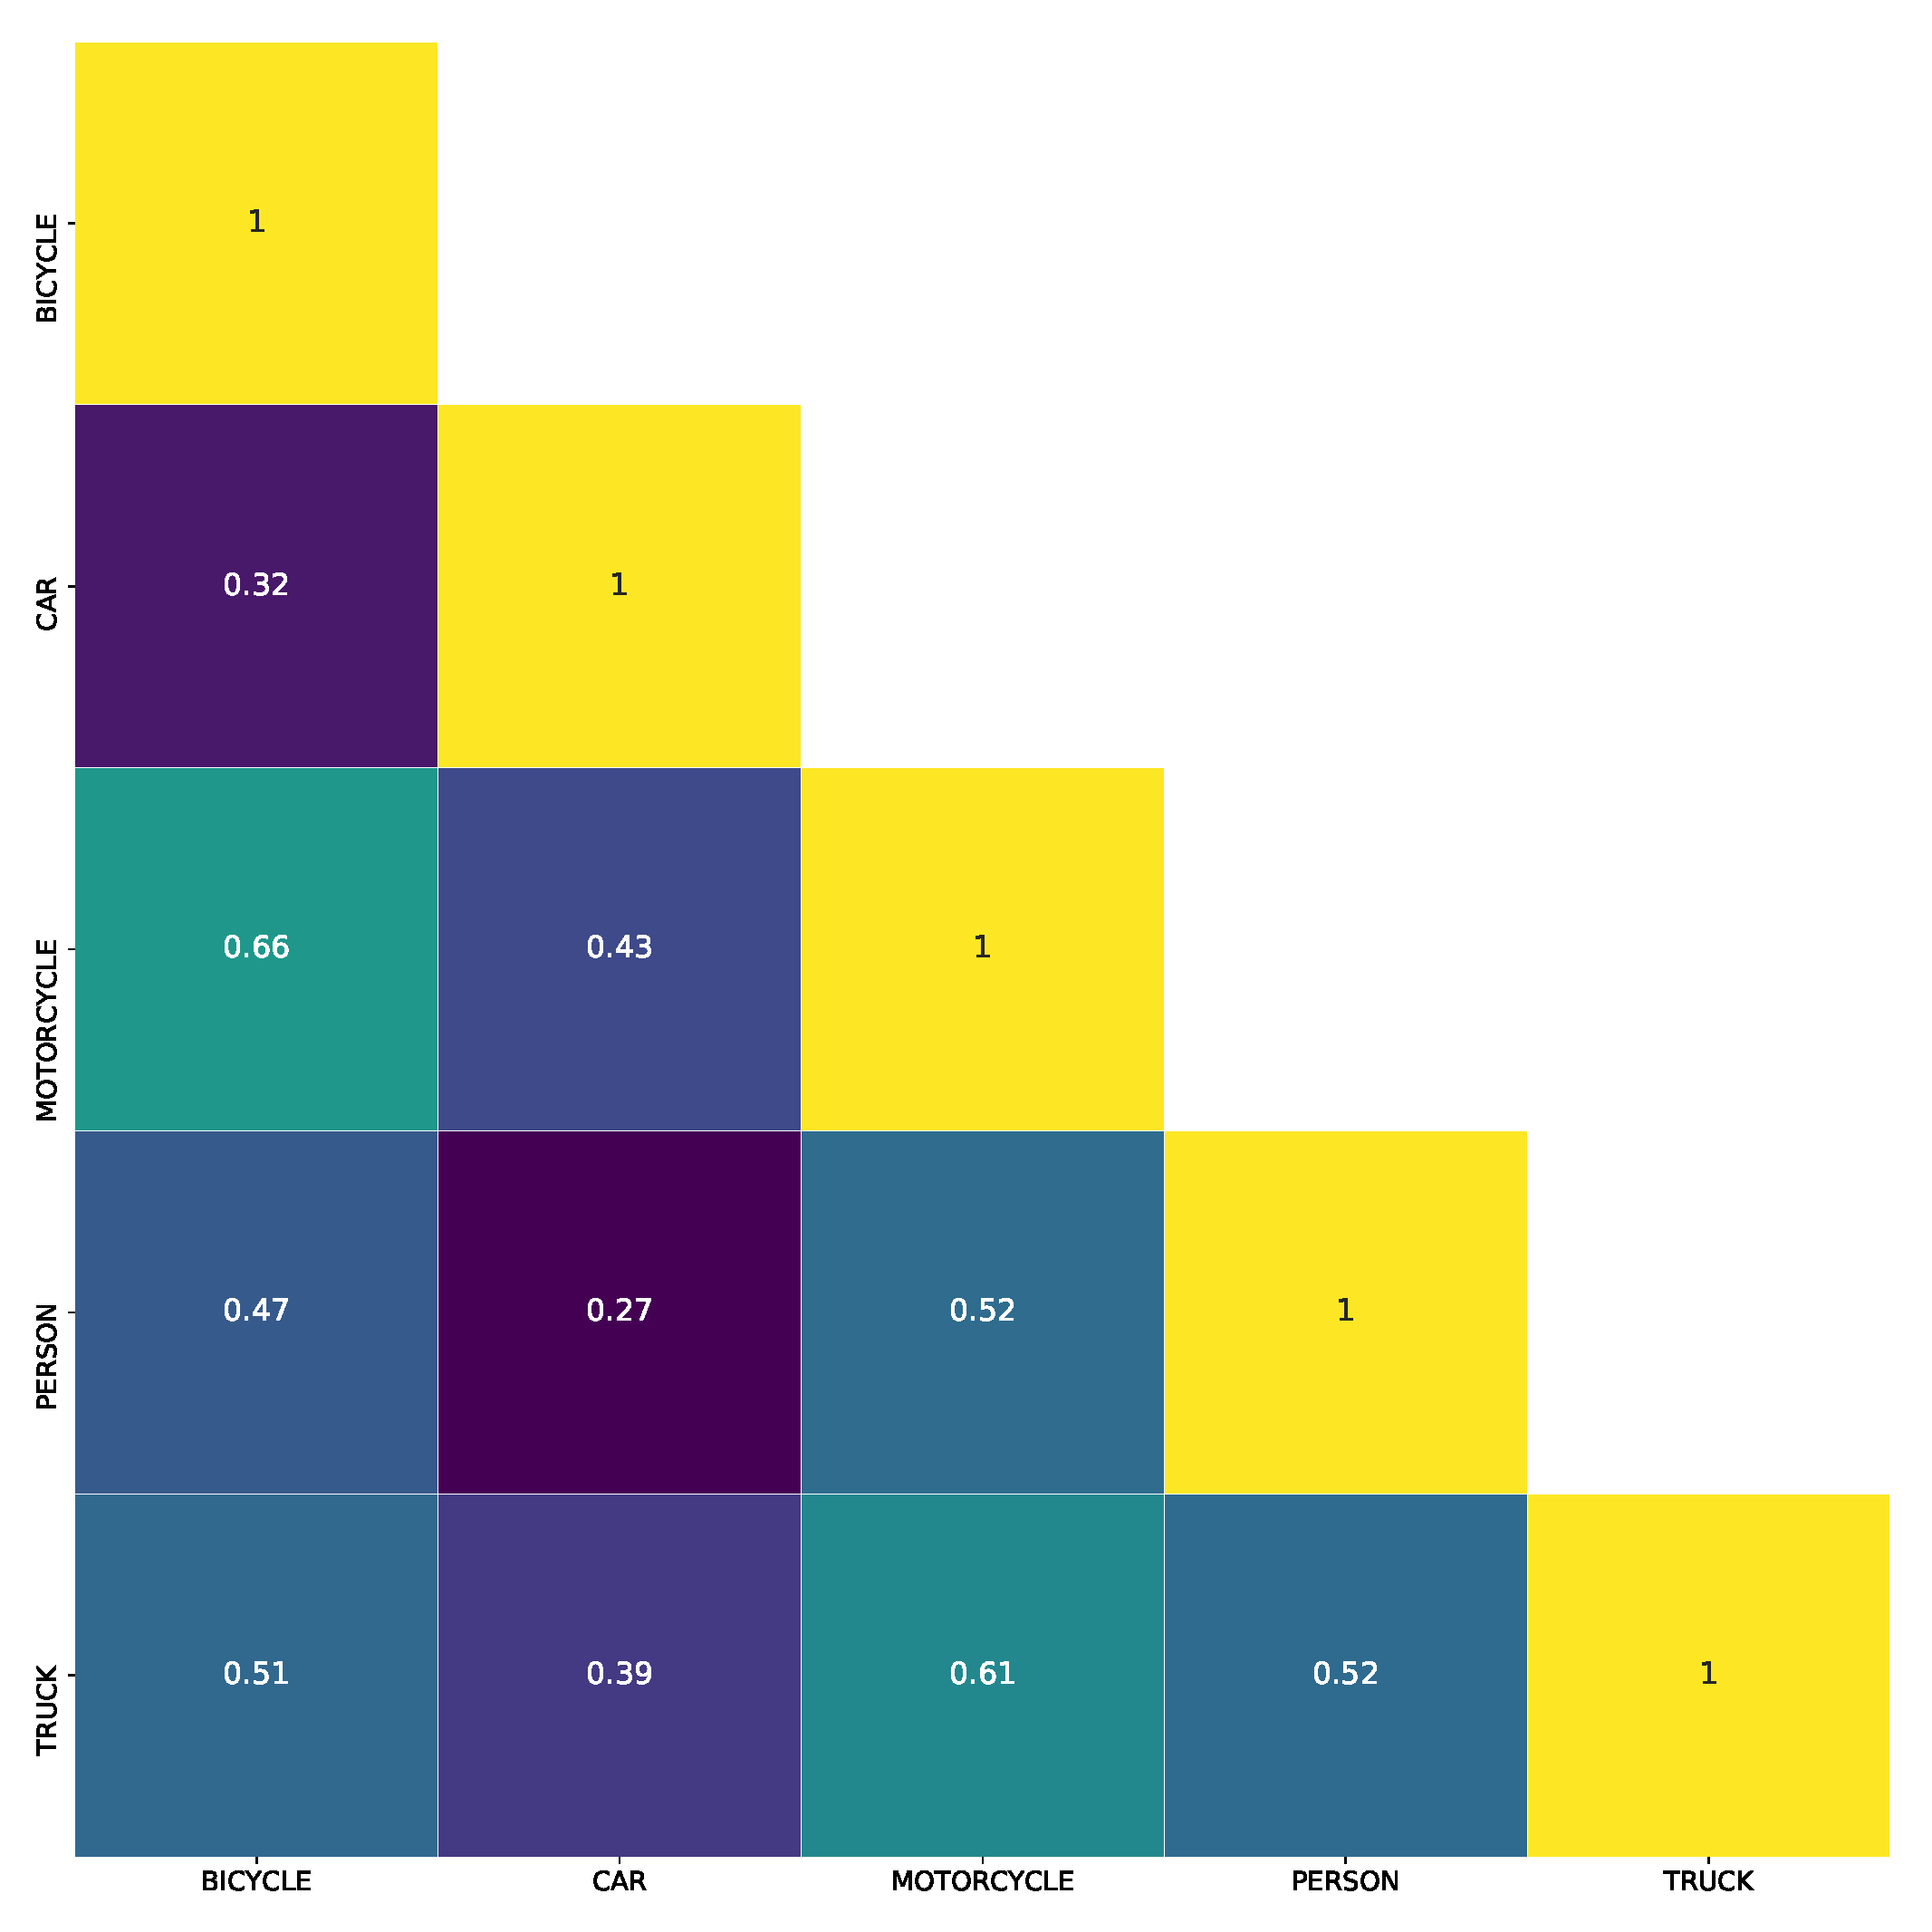
\includegraphics[height=3cm]{imgs/semantic_vocab_traffic_participants_word2vec_internal_similarities.eps}
        }
        \subfloat[\label{subfig:semantic_vocab_traffic_participants_manual_internal_similarities}]{%
            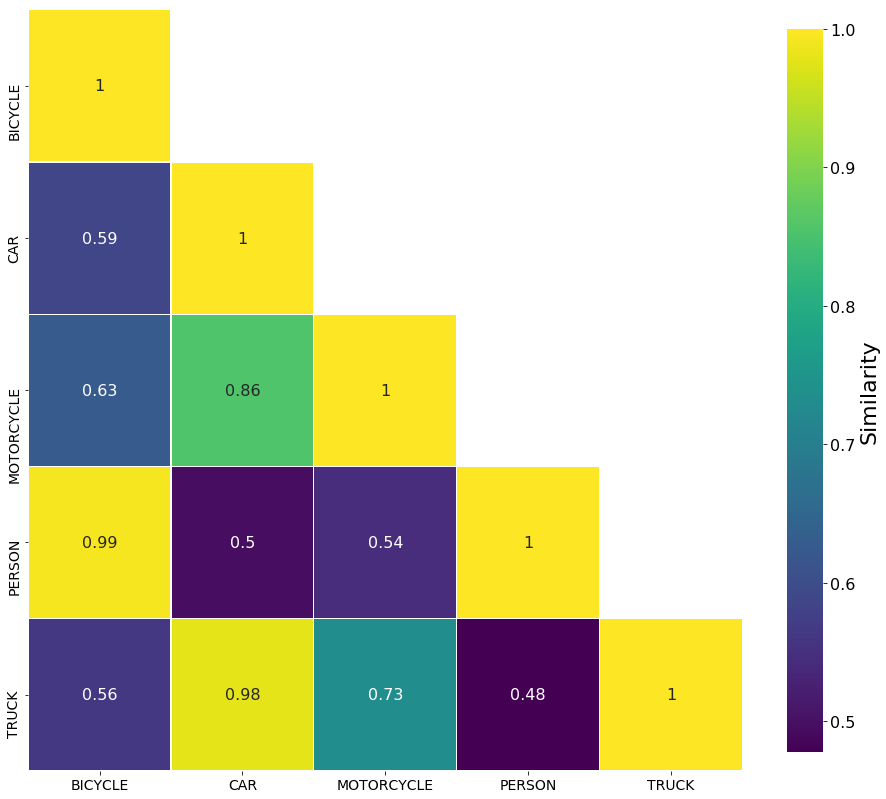
\includegraphics[height=3cm]{imgs/semantic_vocab_traffic_participants_manual_internal_similarities.eps}
        }
    }
    \caption{Pairwise similarities between representative vectors encoding traffic participants in a semantic vector vocabulary.~\protect\subref{subfig:semantic_vocab_traffic_participants_word2vec_internal_similarities} Learned with word2vec~\protect\subref{subfig:semantic_vocab_traffic_participants_manual_internal_similarities} manually designed.}
    \label{fig:semantic_vocab_traffic_participants_internal_similarities}
\end{figure}

As discussed in section~\ref{subsec:what_types_of_data_to_encode_}, semantic similarity for traffic participants is hard to capture intuitively.
We concluded that the general meaning of traffic participants is highly context-dependent, which in turn can only be learned from dynamic driving data or from a text corpus describing traffic situations.
However, such data sets are either not available or do not even exist.
Hence, as a first step towards the goal of encoding semantic similarity, we will therefore encapsulate the similarity between the five classes of traffic participants already discussed in section~\ref{subsec:visual_vocabularies}, namely \emph{Bicycle}, \emph{Car}, \emph{Motorcycle}, \emph{Pedestrian}, \emph{Truck}.
Here, we employ two different approaches: an automated learning approach making use of the well-established word embedding of the word2vec algorithm \parencite{Mikolov2013} trained on the Google News data set and, similar to the semantic vocabulary of traffic signs, manual design, which is only possible due to the small size of our vocabulary.
Word2vec is an unsupervised learning approach generating a word embedding, i.e., vectors representing every word encountered in the training text, where words that appear in similar context, i.e., close proximity within the text, are mapped to similar vectors. 
For our purposes, we simply extract the (\num{300}-dimensional) vectors representing the objects of interest (traffic participants) from the learned vocabulary.
The manually designed semantic vocabulary is generated similarly to the aforementioned vocabulary of traffic signs using the \ac{SPA}'s algebraic operation and the role-filler-pairs approach based on two key properties, which give good yet simple descriptions of the traffic participant's semantic properties: speed and vulnerability represented by randomly chosen atomic vectors \textbf{SPEED} and \textbf{VULNERABILITY}.
Hence, we encode the five classes of traffic participants through

\begin{equation}
\label{eq:semantic_vocab_traffic_participants}
\mathbf{PARTICIPANT} = \mathbf{SPEED} \varoast \varphi(s) + \mathbf{VULNERABILITY} \varoast \varphi(v),
\end{equation}
using the encoding function $\varphi$ from Equation~\eqref{eq:cosin_vec_func}.

Figure~\ref{fig:semantic_vocab_traffic_participants_internal_similarities} depicts the pairwise similarities of both, the semantic vocabulary using word2vec vectors (Fig.~\ref{subfig:semantic_vocab_traffic_participants_word2vec_internal_similarities}) and the manually designed vocabulary vectors (Fig.~\ref{subfig:semantic_vocab_traffic_participants_manual_internal_similarities}).
We observe that the pre-trained word vectors from word2vec are not entirely successful to capture the kind of semantic similarity we are interested in.
While vectors are similar to each other, the individual similarities do not always match our human understanding, especially when considering an automotive context.
For instance, the vector encoding \emph{person} is significantly more similar to the one representing \emph{truck} than to the one representing \emph{car} 
Furthermore, \emph{car} is the traffic participant least similar to \emph{truck}. 

For the manually designed vocabulary (Fig. \ref{subfig:semantic_vocab_traffic_participants_manual_internal_similarities}), results are more convincing.
We are able to achieve a higher similarity between vectors encoding \emph{car} and \emph{truck} as well as \emph{bicycle} and \emph{person} with lower similarities between \emph{person} and \emph{truck} as well as \emph{bicycle} and \emph{truck}.
This vocabulary is also not an ideal representation but gets much closer to the desired semantic structure between these entities in an automotive context. 

\subsection{Visual-semantic vocabularies}%
\label{subsec:visual_semantic_vocabularies}
 
After having created vector vocabularies encoding visual (section~\ref{subsec:visual_vocabularies}) and semantic similarity (section~\ref{subsec:semantic_vocabularies}) structures, we aim to generate a vector vocabulary, which combines both aforementioned similarities in one comprehensive vocabulary.
The idea is that for high or low similarity in both, visual and semantic domain we want the resulting vectors to preserve or even increase that similarity structure.
For a diverging similarity in the two domains, the fusion process should somewhat dilute the two extremes resulting in vectors with medium similarity.
Contrary to other visual-semantic fusion methods, these properties can be achieved employing again the algebraic operations of the \ac{SPA} and the role-filler-pair approach.
Therefore, we randomly choose two additional role vectors, \textbf{VISUAL} and \textbf{SEMANTIC} and construct the visual-semantic vocabulary vectors as
\begin{equation}
\label{eq:visual_semantic_vocab}
\mathbf{VISUALSEMANTIC} = \mathbf{VISUAL} \varoast \mathbf{V} + \mathbf{SEMANTIC} \varoast \mathbf{S},
\end{equation}
where \textbf{V} and \textbf{S} are placeholders for the visual and semantic vocabulary vectors to be fused.
Given the mathematical properties of the \ac{SPA}'s algebraic operations (cf.\ chapter~\ref{chap:introduction_to_vsas}), this fusion procedure guarantees that for two similar vectors in either of the input domains, the resulting visual-semantic vectors will preserve that similarity.

\subsubsection{Traffic signs}%
\label{ssubsec:traffic_signs}

\begin{figure}[t]
    \centering
    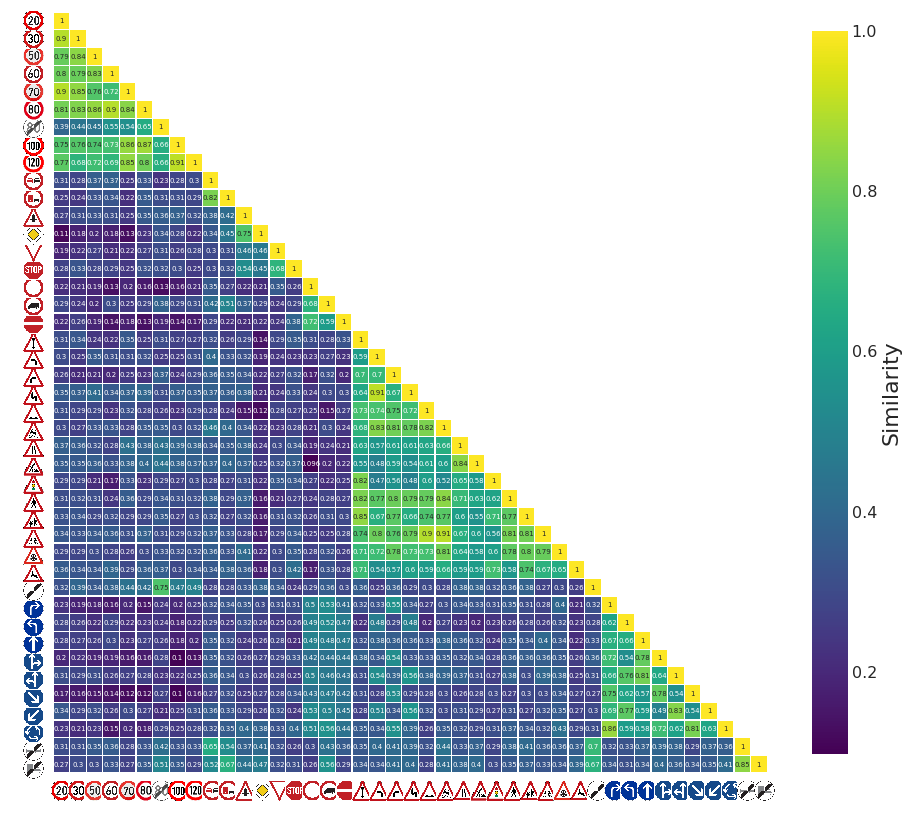
\includegraphics[width=1.0\linewidth]{imgs/visual_semantic_vocab_traffic_signs_internal_similarities.eps}
    \caption{Pairwise similarities between vectors encoding traffic signs in a visual-semantic vocabulary.}
    \label{fig:visual_semantic_vocab_traffic_signs_internal_similarities}
\end{figure}

Figure~\ref{fig:visual_semantic_vocab_traffic_signs_internal_similarities} shows the pairwise similarities of the visual-semantic vocabulary vectors representing traffic signs.
We observe that opposite similarities from the input domains are smoothed out through the convolution-based fusion process.
For instance, the strong visual similarity between the traffic sign indicating \enquote{Priority ahead} and all attention signs (triangular shape, red border, black symbol in the middle), which has been clearly visible in Fig.~\ref{fig:visual_vocab_traffic_signs_internal_similarities}, does not correspond to a large semantic similarity and was canceled during the fusion procedure.
The same holds true for the clearing signs as well as for the similarities between signs indicating \enquote{No entry trucks} and \enquote{roundabout} and the speed limits.
On the other hand, for those traffic signs with high semantic similarity such as between signs indicating overtaking rules for trucks and the sign indicating no entry for trucks, this similarity is preserved in the joint visual-semantic vocabulary. 
Particularly for the speed limits, we observe that a high similarity in both domains translates into a high joint similarity, whereas in other cases, the manually designed semantic similarity is partly \enquote{overwritten} with the visual information.
In general, many signs from different groups with very low semantic similarity (the dark blue block in the bottom left of Fig.~\ref{fig:visual_semantic_vocab_traffic_signs_internal_similarities}) are increased by the visual part. 

\subsubsection{Traffic participants}%
\label{ssubsec:traffic_participants}

\begin{figure}[t]
    \centering
    \resizebox{.9\textwidth}{!}{%
        \subfloat[\label{subfig:visual_semantic_vocab_traffic_participants_word2vec_internal_similarities}]{%
            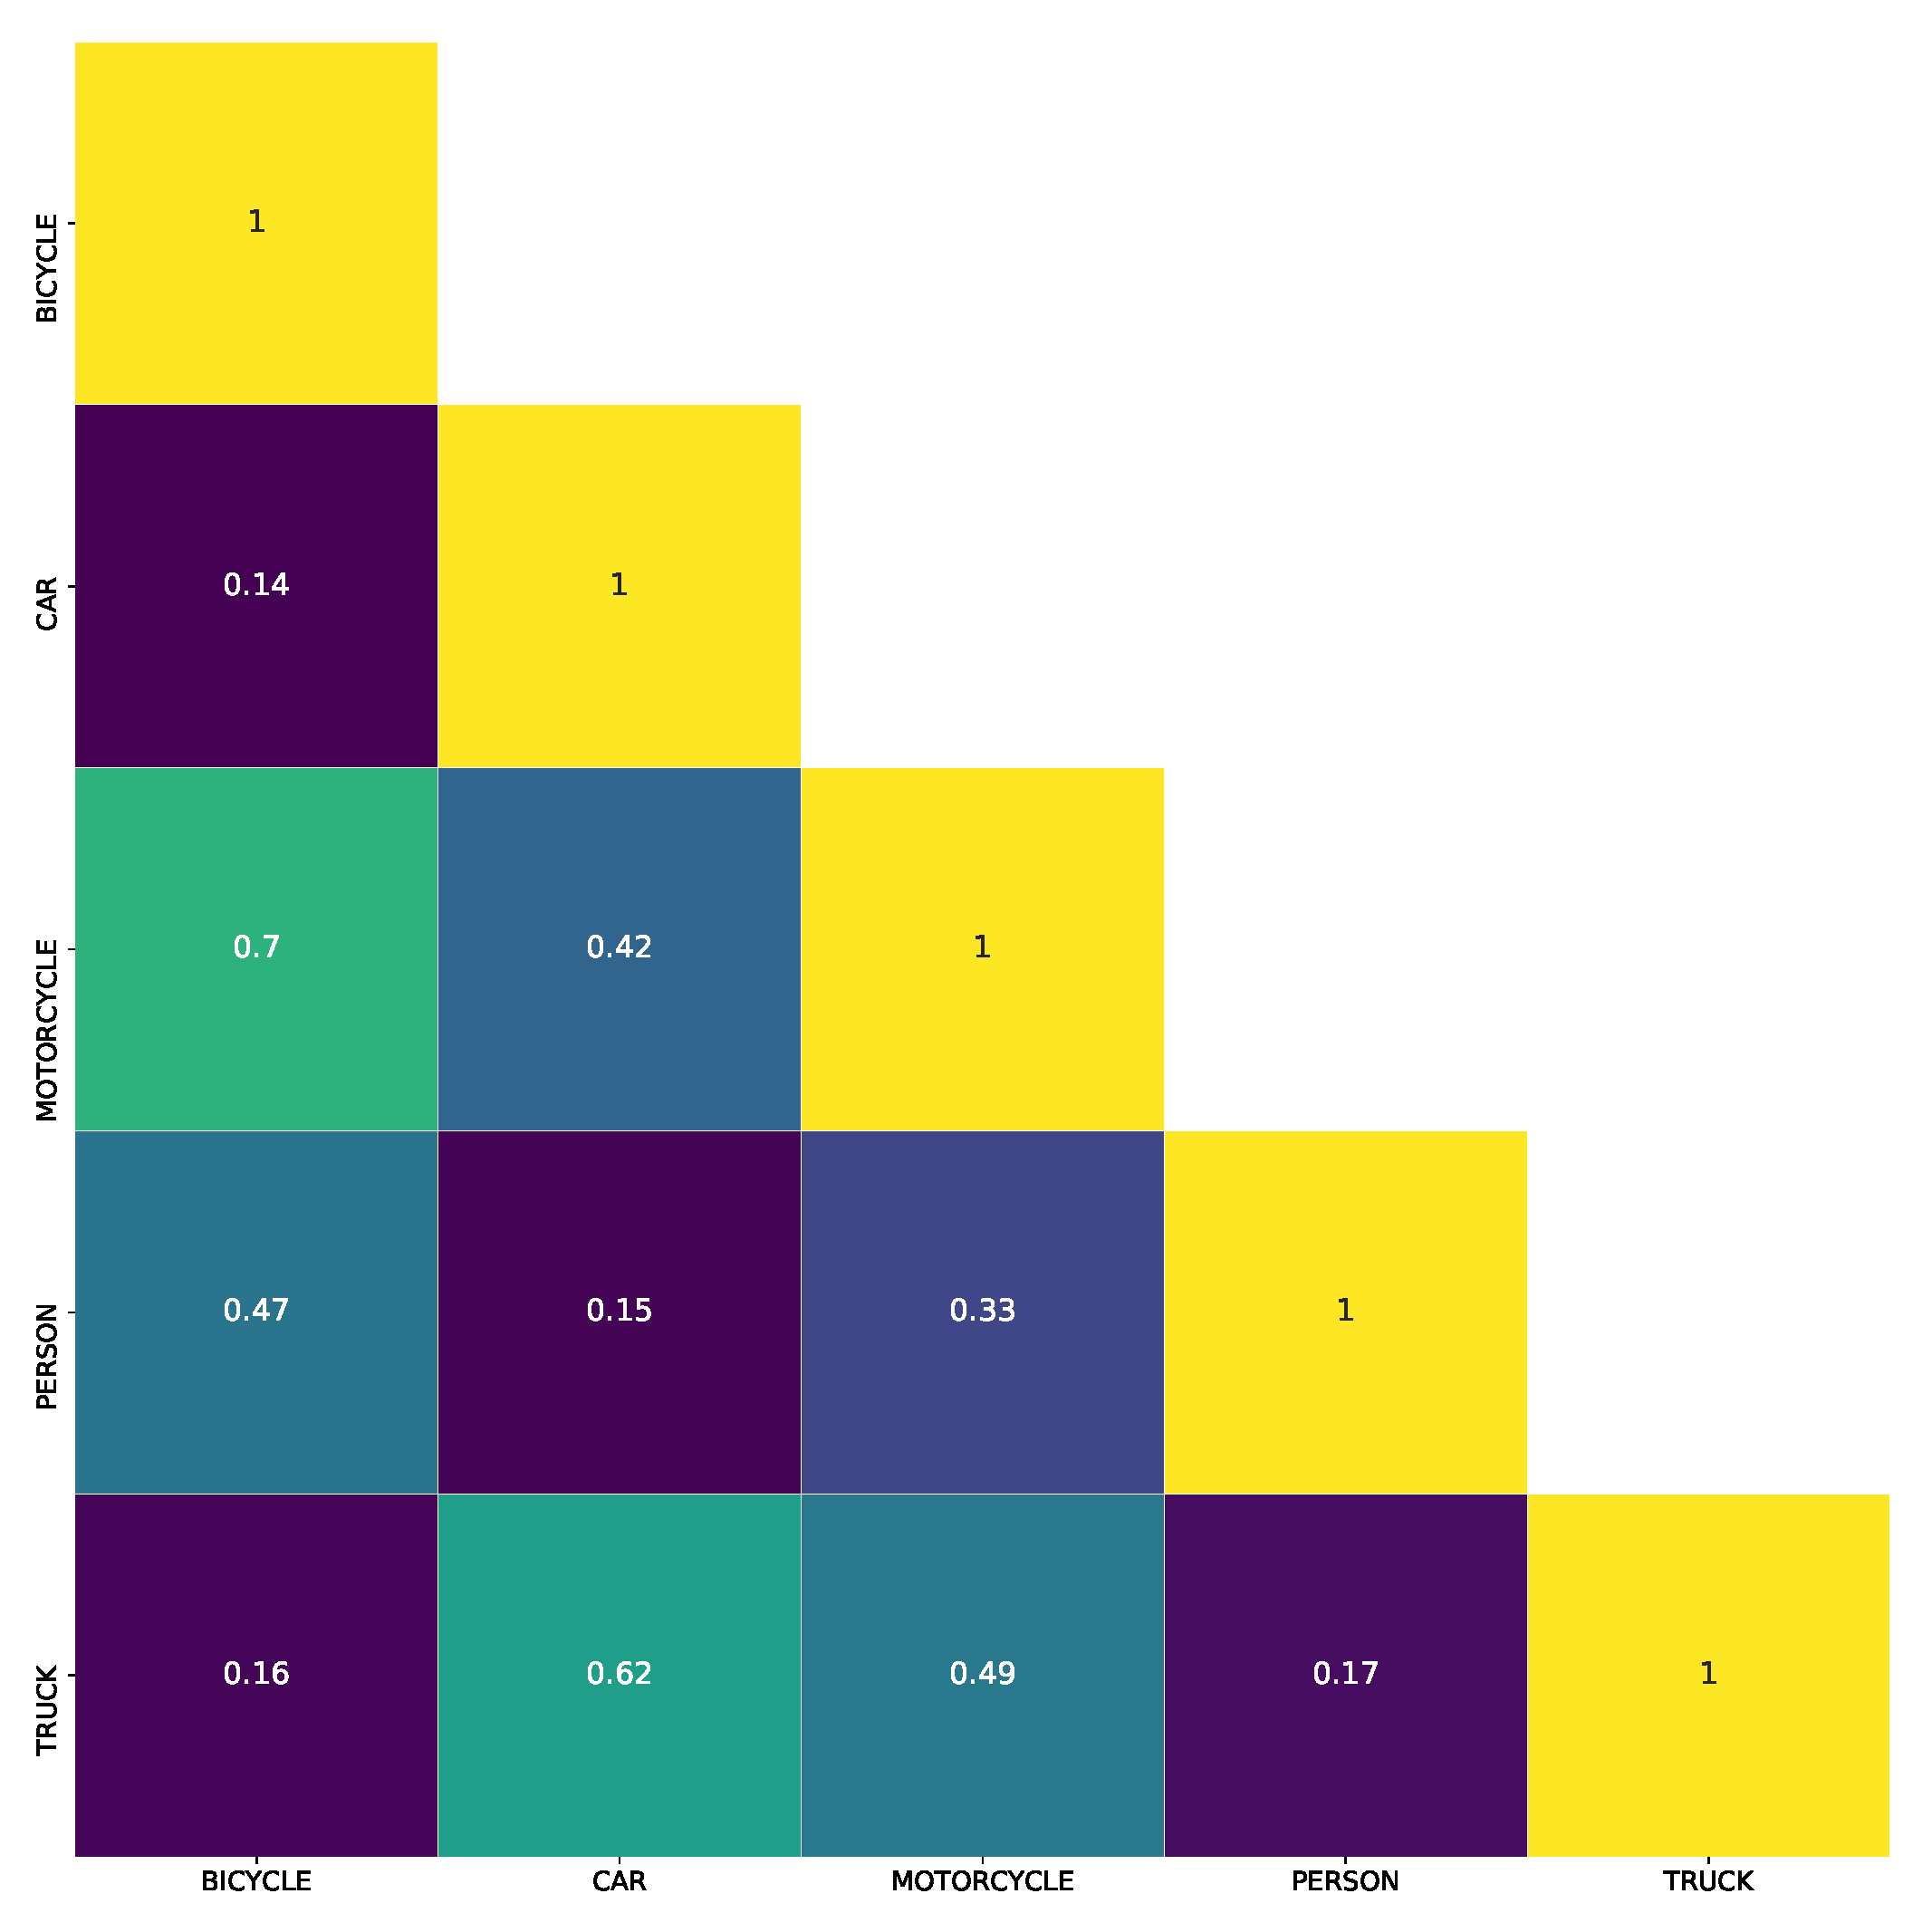
\includegraphics[height=3cm]{imgs/visual_semantic_vocab_traffic_participants_word2vec_internal_similarities.eps}
        }
        \subfloat[\label{subfig:visual_semantic_vocab_traffic_participants_manual_internal_similarities}]{%
            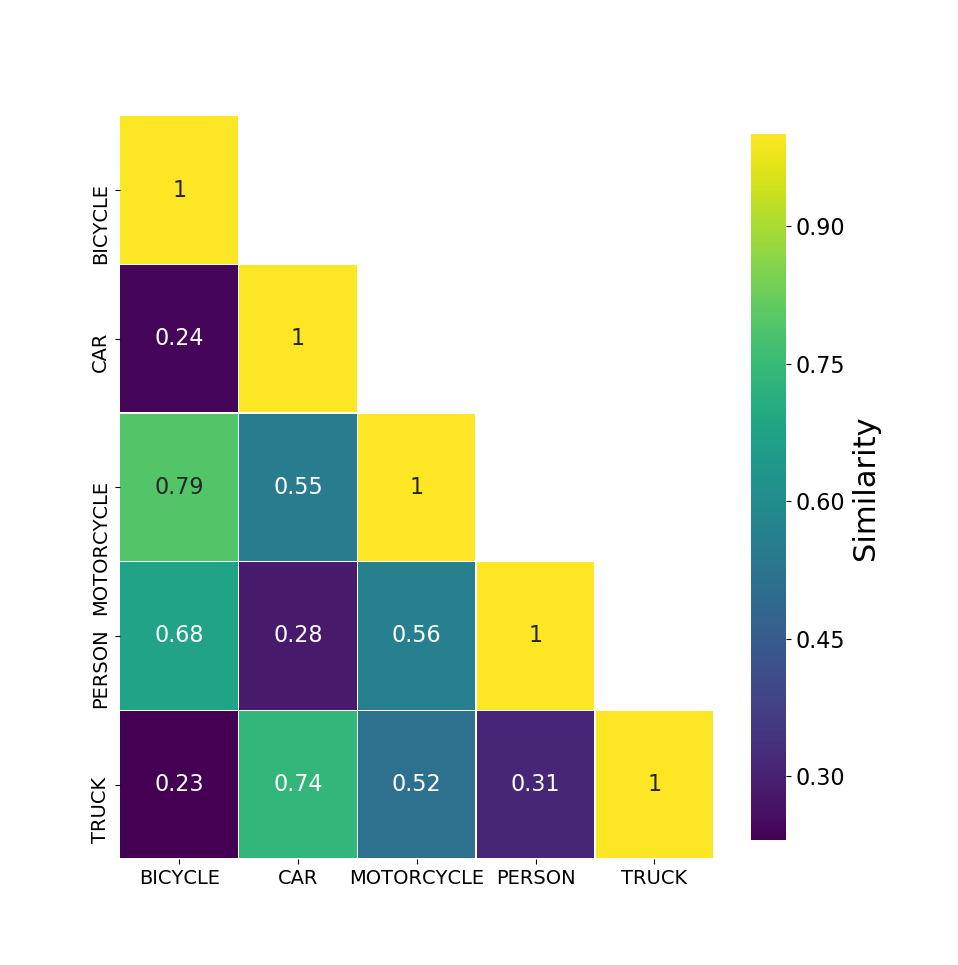
\includegraphics[height=3cm]{imgs/visual_semantic_vocab_traffic_participants_manual_internal_similarities.eps}
        }
    }
    \caption{Pairwise similarities between vocabulary vectors encoding traffic participants in a visual-semantic vocabulary, where the semantic part is~\protect\subref{subfig:semantic_vocab_traffic_participants_word2vec_internal_similarities} learned with word2vec~\protect\subref{subfig:semantic_vocab_traffic_participants_manual_internal_similarities} manually designed.}
    \label{fig:visual_semantic_vocab_traffic_participants_internal_similarities}
\end{figure}

In section~\ref{subsec:semantic_vocabularies}, we created two semantic vocabularies, which have been learned with word2vec and manually designed.
Figure~\ref{fig:visual_semantic_vocab_traffic_participants_internal_similarities} depicts the pairwise similarities of two visual-semantic vocabularies, where the two different vocabularies from section~\ref{subsec:semantic_vocabularies} are used for the semantic part.
We observe fusion results similar to those for the visual-semantic traffic sign vocabulary, where opposite similarities from the input domains are smoothed out through the convolution-based fusion process while differences in semantic structure between the two methods remain visible in the complete vocabulary.
Consequently, the visual-semantic encoding based on manually designed semantics appear to be a convincing vector representation for the similarity structure expected for traffic participants in an automotive context.

\subsection{Summary on vocabularies}%
\label{subsec:summary_on_vocabularies}

In this section, we investigated several options of generating a suitable vector vocabulary for entities of interest in an automotive context.
We have shown a way of learning a visual structure for two classes of categories appearing in an automotive context, namely traffic signs and traffic participants using \acp{CNN}.
Furthermore, we were able to create a learned semantic vocabulary for traffic participants, but not traffic signs due to lack of suitable training data sets.
Hence, we designed the semantic vocabulary for traffic signs manually using the mathematical properties and algebraic operations of the \ac{SPA}.
Furthermore, we also generate an alternative semantic vocabulary for traffic participants as a baseline to compare the learned semantic structure, which has not been adapted to the automotive context, to.
Finally, we successfully generated a visual-semantic vocabulary encapsulating both, visual and semantic similarity by using the \ac{SPA}'s algebraic operations and the role-filler-pair approach.
This visual-semantic vocabulary appears to represent the expected similarity structure between the entities of interest in automotive context.

It is worth noting however that the manual generation process of the semantic vocabularies, as mentioned in~\ref{subsec:basic_random_vocabularies}, imposes a significant amount of design choices biased by the human engineer.
However, the choice of generating some of the semantic vectors in this context manually is due to the fact that on the one hand, the vocabulary is comparatively small while on the other hand, there are no suitable data sets available to learn the desired semantic structure from.
Furthermore, the described procedure to fuse visual and semantic similarities into one coherent vocabulary is only one of several available options.
It would have also been possible to try to automatically learn such a fusion process by projecting the visual vocabulary to the semantic one by combining visual properties and language descriptions like for instance in \textcite{Karpathy2017}.
However, such a learning approach again would require a suitable, sufficiently large data set, which in turn is not available for the entities investigated here.

Finally, the process of generating structured representations from an available vocabulary created with any of the techniques described in this section is independent from the particular vocabulary at hand.
Hence, although it seems intuitive and useful to encode similarities of potential interest to the task to be solved using the vector representation, it remains to be seen, if using a vocabulary encapsulating any form of similarity actually improves task performance.
Furthermore, the choice which similarity structure to use naturally appears to be heavily task-dependent.
Thus, we will investigate the influence of the vocabulary structure on the task performance for the selected task of driving context classification in chapter~\ref{chap:driving_context_classification} by simply evaluating the same models with changing underlying vocabularies.

\section{Representation generation stage}%
\label{sec:representation_generation_stage}

After having created a vector vocabulary suitable for a specific application of interest as shown in section~\ref{sec:preprocessing_stage_generating_a_vocabulary}, we focus our attention in this section to the second stage of the encoding process proposed by \textcite{Gallant2013}, the \emph{representation generation stage}.
This second step is the process of actually generating structured vector representations from a given vocabulary of atomic vectors.
As mentioned by \textcite{Gallant2013}: \enquote{Although the preprocessing and output computation stage can involve significant machine learning, there are reasons for the representation generation stage to \emph{avoid} machine learning}.
Using machine learning in the stage of representation generation means to adjust the representation to the specific set of applications, which restricts them to be used for different, but related sets of problems.
Furthermore, involving learning in the representation generation might slow down the whole system prohibiting practical usage of the representation in application scenarios.
However, in certain situations it could make sense to involve a learning step at the representation generation stage, for example if the system should detect novelties and assign them to new vectors or representations and/or needs to memorize them.

In this work however, we will focus our efforts mainly on representations which are manually designed without involving machine learning models.
Thereby, we aim to generate representations that are general enough to be applied to a variety of different problems with only moderate modifications necessary when being applied to one particular task.
One crucial aspect in the field of automotive scene representation is encoding dynamic data such as positions or velocities, which constitutes a significant part of the situational context.
This context is essential for the representation to capture the semantics of the scene and gather a comprehensive understanding of the situation at hand.
Depending on the application, different requirements on such a representation might be necessary.
For instance, for some applications it might be necessary that the encoded numerical values need to be decoded back out exactly from the representing vector while for others an approximate recovery might be sufficient.
Other tasks might demand for the representational vectors to have unit length independent from the encoded value.
We therefore investigate several possible options of how to encode numerical values in semantic vectors focusing on different aspects of possible requirements.

Encoding numerical values, although an important one, is only one aspect of representing automotive scenes in high-dimensional vectors.
The second crucial aspect of the representation generation stage is that of how to build up vectors representing structured information and complex interrelations encountered in automotive scenes.
We need to combine several pieces of information into one or a set of scene vectors of fixed length representing the semantics of the situation.
We will investigate how the \ac{SPA}'s algebraic operations can be used to combine numerical and symbol-like information to build such complex representations.

However, given the mathematical properties of \acp{VSA} in general and the \ac{SPA} in particular, there are natural limitations to the amount of information that can be encoded in such a vector representation.
Every algebraic operation, addition and circular convolution, will introduce a certain amount of noise into the representation, which imposes the functional demand for a clean-up memory (cf.\ chapter~\ref{chap:introduction_to_vsas}) for some applications.
These limitations are actually not a flaw of such architectures, but rather a feature for being able to model limitations of cognitive functions of living beings, who are also not able to store unlimited amounts of information.
The limitations of the modeling architecture are strongly connected to the chosen dimension of the underlying vector space.
Therefore, we will finally analyze what kind of limitations these architectures impose on us and how much information can effectively be encoded in such a vector representation before noise reaches a critical level.

\subsection{Different vector representations for numerical values}%
\label{subsec:different_vector_representations_for_numerical_values}

In this section, we investigate different approaches to map numerical information to semantic vectors.
We have already seen one simple option for such an encoding in section~\ref{subsec:semantic_vocabularies}, where we used the function $\varphi$ from Equation~\eqref{eq:cosin_vec_func}.
Here, we will show a more complex adoption of this encoding again making use of the sine and cosine functions alongside two more possibilities of how to represent numerical values.

\subsubsection{Sine-Cosine-based representations}%
\label{ssubsec:sine_cosine_based_representations}

The idea behind using the sine and cosine functions to encode numerical values in high-dimensional vectors is their property of adding up to \num{1} when being squared, the Pythagorean identity
\begin{equation}
\label{eq:pythagorean_identity}
\sin^{2}(x) + \cos^{2}(x) = 1.
\end{equation}

For the simple encoding given in Equation~\eqref{eq:cosin_vec_func} 
\begin{equation}
\abb{\varphi}{\mathbb{R}}{\mathbb{R}^{D}}{x}{\left(\sin(x), \cos(x), 0, \ldots, 0\right)},
\tag{\eqref{eq:cosin_vec_func} revisited}
\end{equation}
Equation~\eqref{eq:pythagorean_identity} leads to the resulting vector $\varphi(x)$ having unit length, which is a desirable feature for many representations.

Since most of the dynamic data to be encoded in automotive context such as positions and velocities is two-dimensional, we also show a more complex adaptation of this simple trigonometrical encoding for two numerical values using different spatial frequencies and offsets.
Therefore, we define the following auxiliary functions
\begin{align}
    &\abb{f_{\left(m,i\right)}}{\mathbb{R}^2}{\mathbb{R}^4}{\left(x,y\right)}{\left(\cos\frac{m\cdot \pi + x}{i + 1}, \sin\frac{m\cdot \pi + x}{i + 1}, \cos\frac{m\cdot \pi + y}{i + 1}, \sin\frac{m\cdot \pi + y}{i + 1}\right)}, \label{eq:cos_aux_1} \\
    &\abb{\psi_i}{\mathbb{R}^2}{\mathbb{R}^4}{\left(x,y\right)}{\left(f_{\left(0,i\right)}\left(x,y\right), f_{\left(\frac{1}{2},i\right)}\left(x,y\right), f_{\left(1,i\right)}\left(x,y\right), f_{\left(\frac{3}{2},i\right)}\left(x,y\right)\right)} \label{eq:cos_aux_2}
\end{align}
and obtain the final vector representation of two-dimensional values via the function 
\begin{equation}
\label{eq:cosin_2d_enc}
\abb{\lambda}{\mathbb{R}^2}{\mathbb{R}^D}{\left(x,y\right)}{\frac{1}{\sqrt{\frac{D}{2}}}\left(\psi_0\left(x,y\right), \cdots, \psi_{\frac{D}{16}-1}\left(x,y\right)\right).}
\end{equation}

The encoding $\lambda\left(x, y\right)$ leads to non-zero vectors having unit length with information distributed over all elements (in contrast to a simple encoding like $\left(x, y, 0 \ldots, 0\right)$).
Although for both trigonometrical encoding schemes shown here there is a way of decoding back out the input values exactly from resulting vector by using either the inverse trigonometrical functions or the $\atantwo$ function, both approaches have certain drawbacks.
For instance, the simple encoding (cf.\ Equation~\eqref{eq:cosin_vec_func}) uses only two of a typically large number of dimensions and thus somewhat neglects the architectural strength of \acp{VSA} being \emph{distributed} representations.
On the other hand, the encoding of two-dimensional values based on different spatial frequencies and offsets of the trigonometrical functions uses all of the available dimensions, but is constructed for vector space dimensions being a multiple of \num{16}.
Although this is true for all sufficiently large powers of \num{2} such as $512=2^{9}, 1024=2^{10}, \ldots$ it still imposes significant restrictions on the potential dimensions of the vector spaces to be used.

\subsubsection{Scalar multiplication encoding}%
\label{ssubsec:scalar_multiplication_encoding}

\begin{figure}[t]
    \centering
    \subfloat[\label{subfig:scalar_encoding_decoding_rmse}]{%
        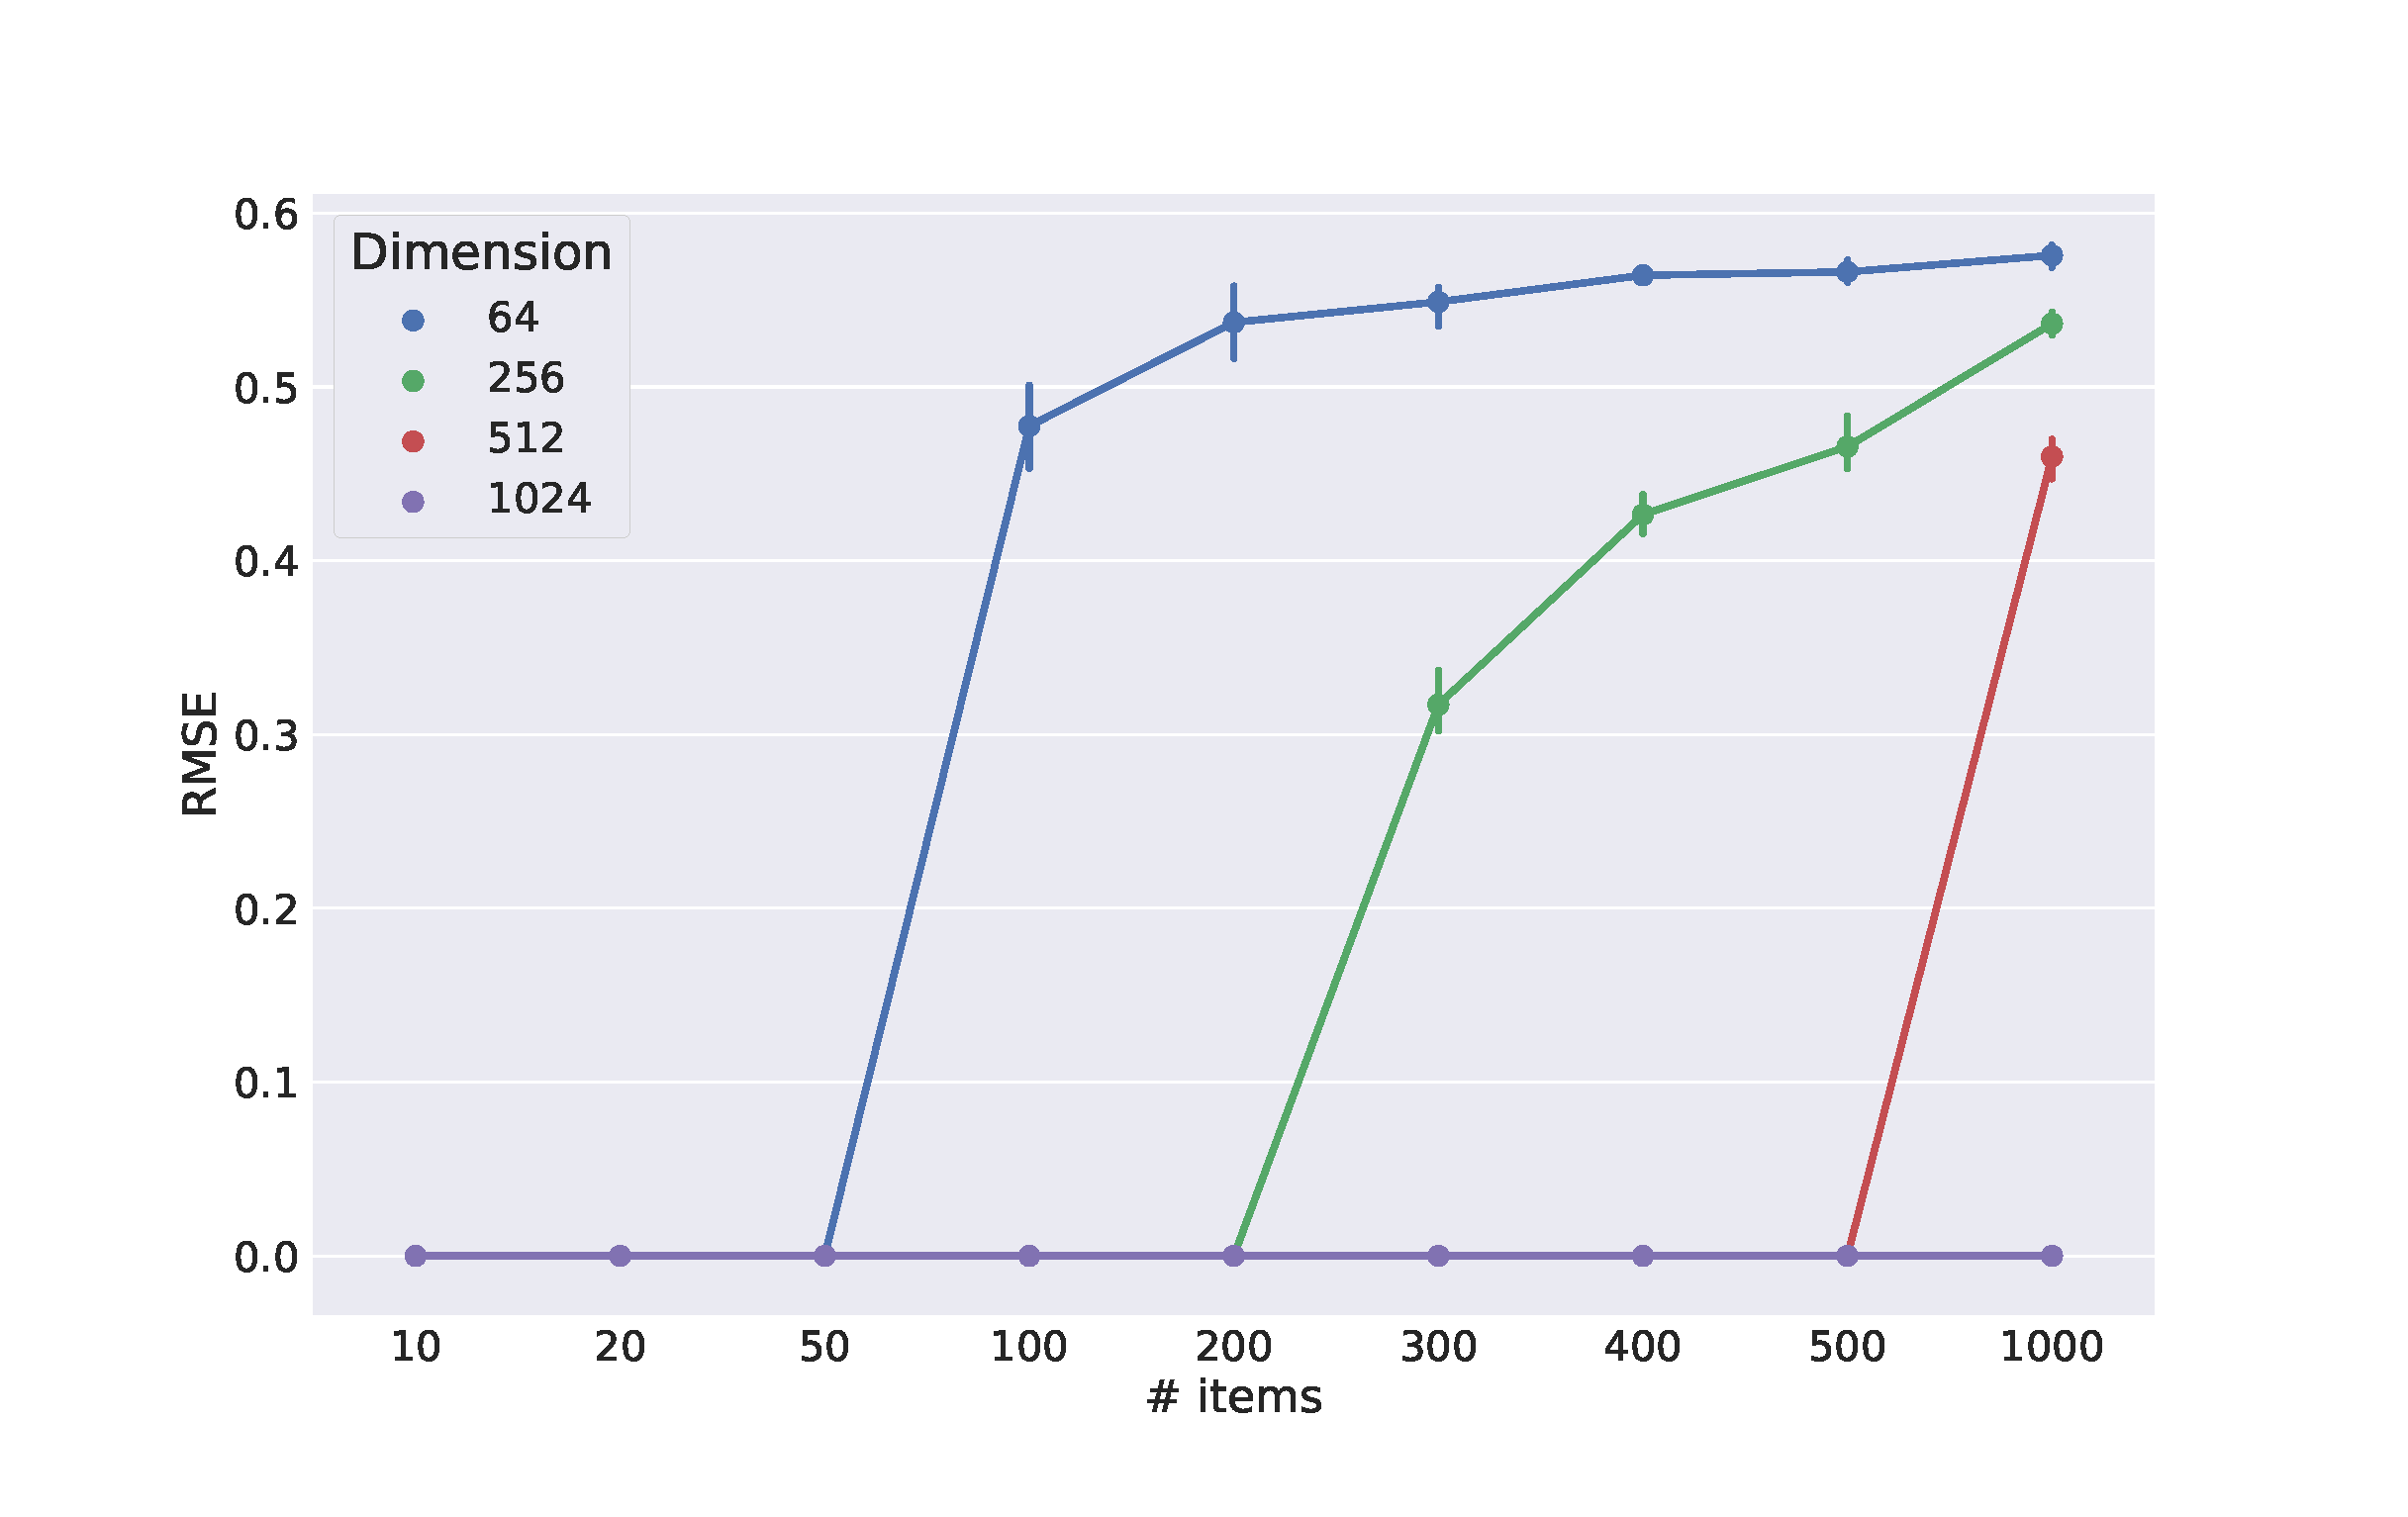
\includegraphics[width=0.5\linewidth]{imgs/scalar_encoding_decoding_rmse.eps}
    }
    \subfloat[\label{subfig:scalar_encoding_norm}]{%
        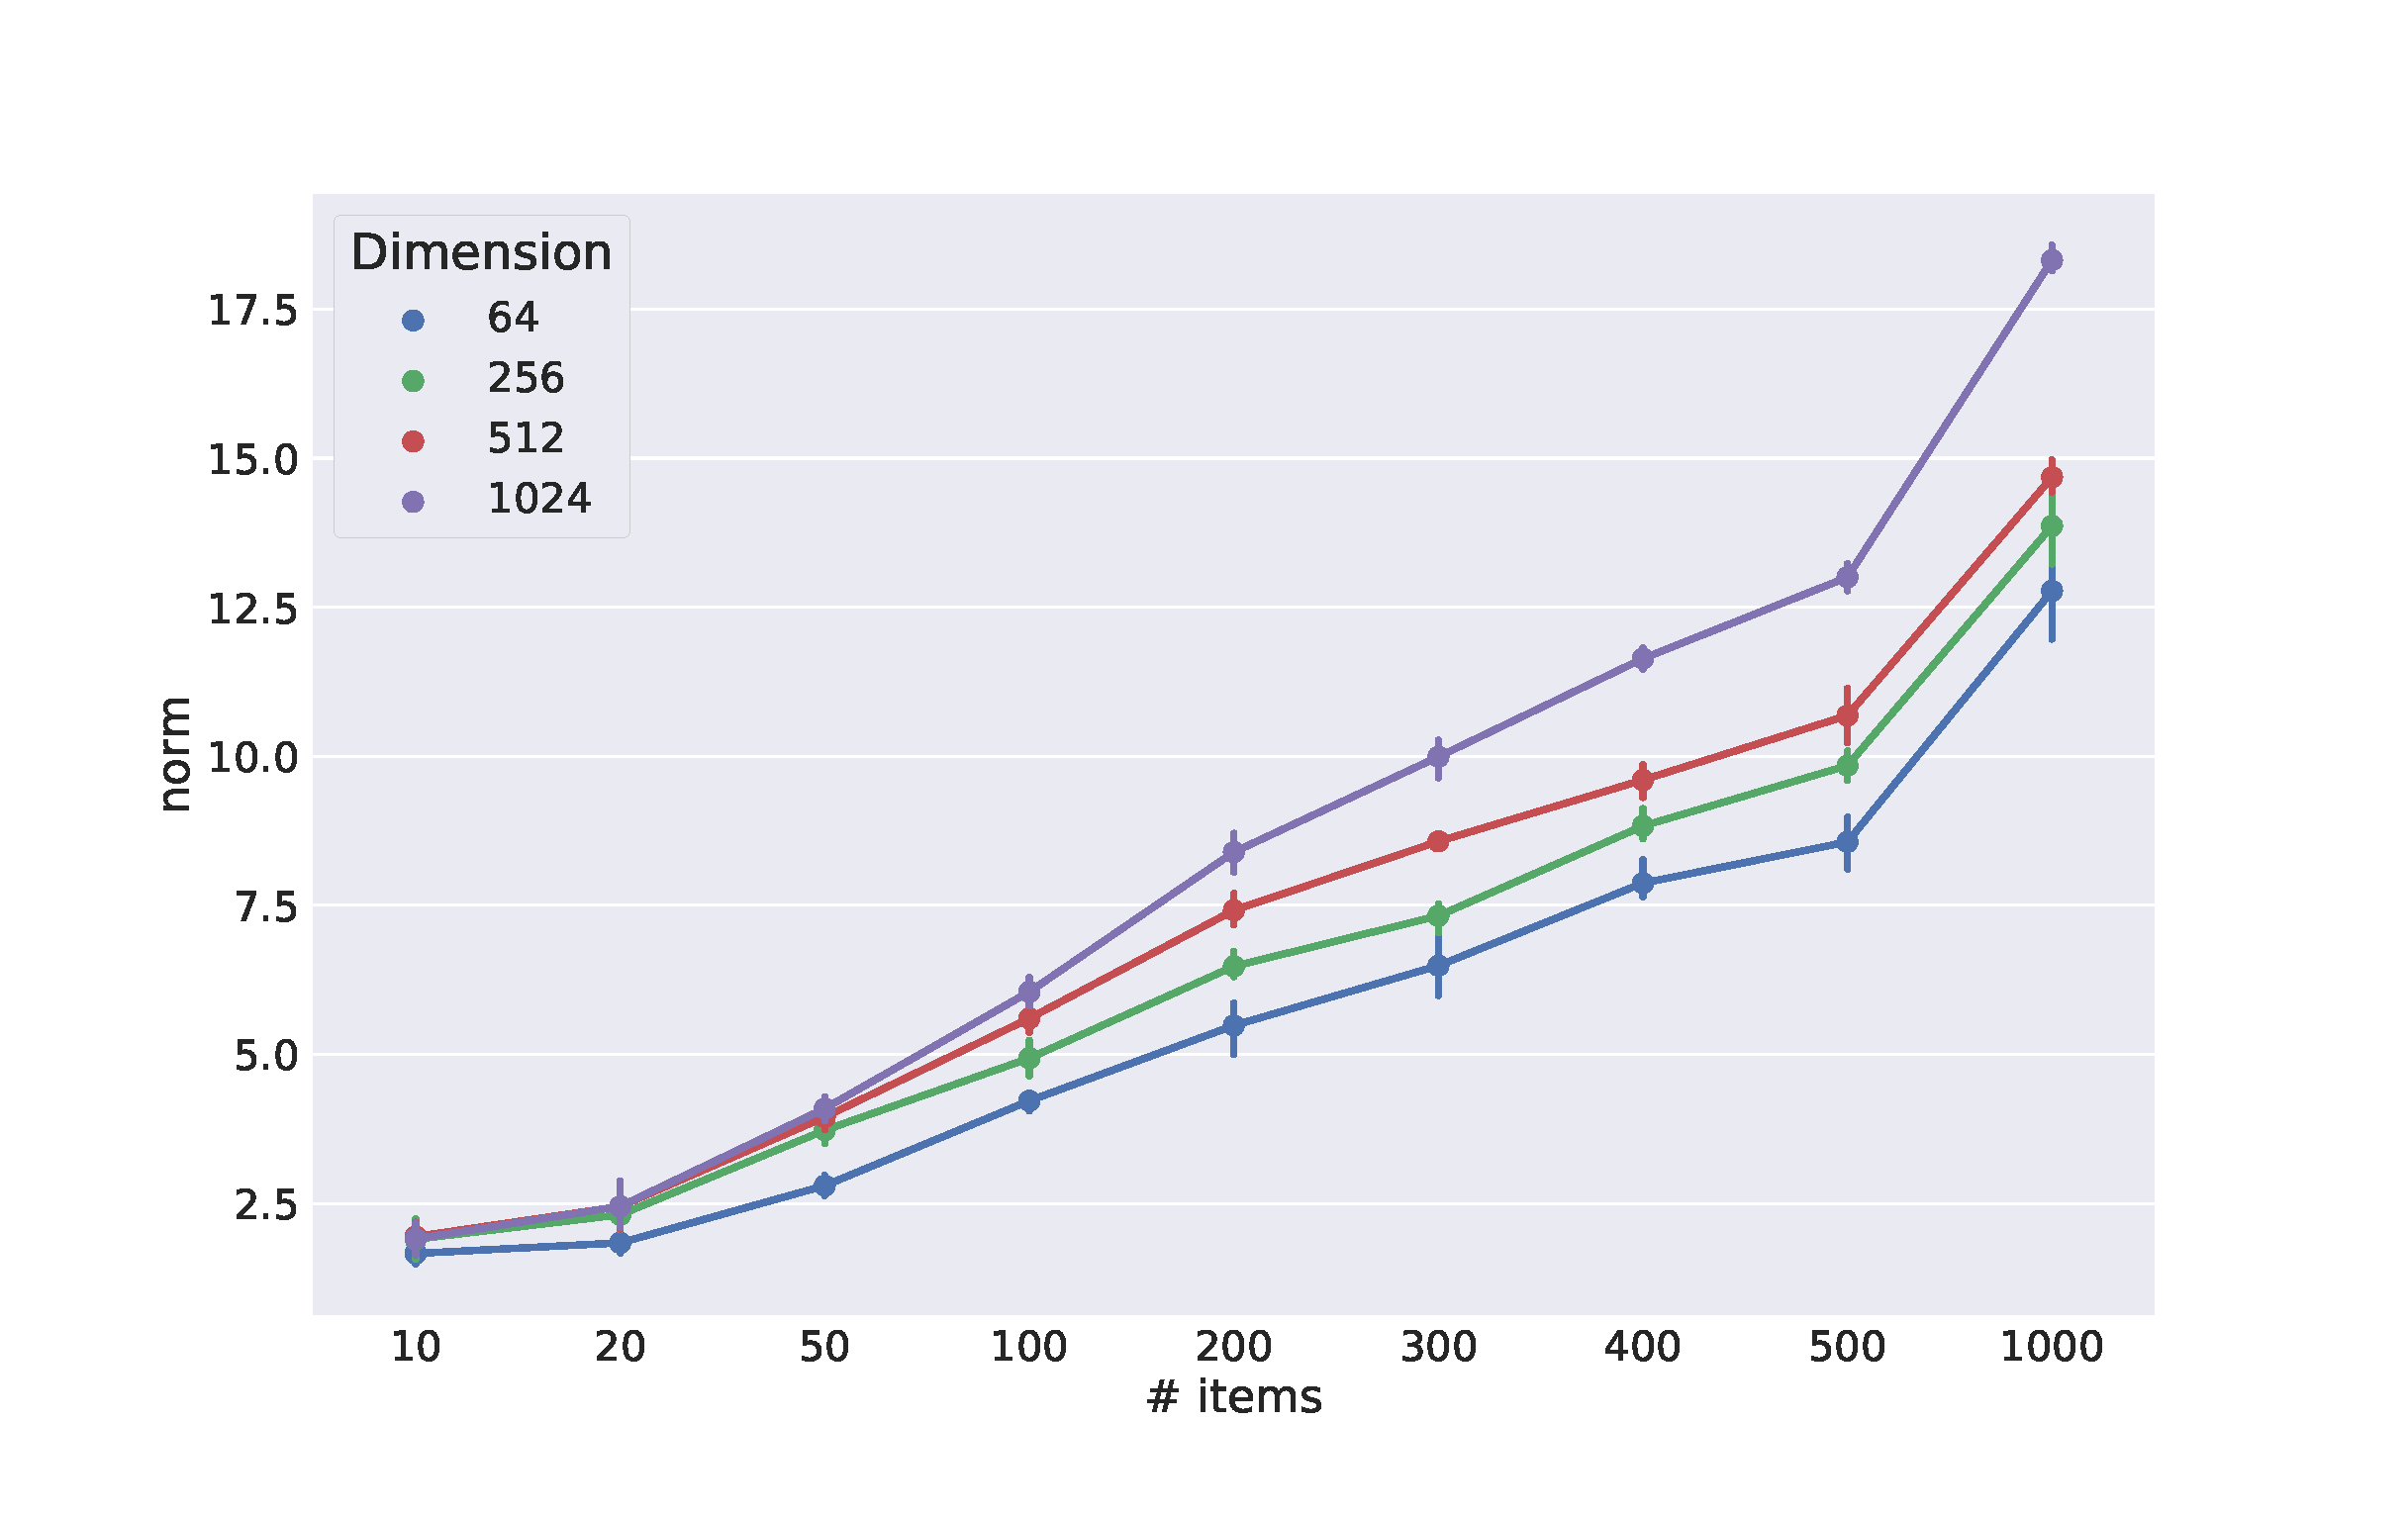
\includegraphics[width=0.5\linewidth]{imgs/scalar_encoding_norm.eps}
    }
    \caption{Properties of the simple scalar multiplication encoding of numerical values in vectors.~\protect\subref{subfig:scalar_encoding_decoding_rmse} shows the \ac{RMSE} when decoding back out an approximation of the original numerical values from the vector representation.~\protect\subref{subfig:scalar_encoding_norm} shows the norm of the representation vectors.}
    \label{fig:scalar_multiplication_encoding}
\end{figure}
Apart from encoding numerical values in vectors as the only non-zero elements within a vector containing only zero elements elsewhere, possibly the simplest encoding is to (for instance, randomly) choose vectors representing the desired entity/unit to be encoded and simply multiply all elements of that vector with the number the vector should represent.
Hence, to encode a sequence $a_{1}, \ldots, a_{n}$ of numerical values in vectors, we create a vocabulary of vectors $\mathcal{V}=\left\{ \mathbf{X}_{1}, \ldots, \mathbf{X}_{n} \right\}$ representing the corresponding units and multiply them by the scalar values with the vectors representing the units $a_{i}\cdot \mathbf{X}_{i}$.
Finally, summing up all of these vectors generates one single vector encoding all of the numerical values $a_{1}, \ldots, a_{n}$ 
\begin{equation}
\label{eq:scalar_mult_encoding}
\mathbf{V} = \sum\limits_{i=1}^{n} a_{i}\cdot \mathbf{X}_{i}. 
\end{equation}

For $\mathbf{X}_{i} = \left(x_{i0}, \ldots, x_{iD-1}\right)^{\intercal}$, this encoding is equivalent to the linear map given by the matrix $ \mathbf{M} $ consisting of the elements of the vectors $ \mathbf{X}_{i}$ column-wise concatenated

\begin{equation}
\label{eq:scalar_encoding_linear_map}
\mathbf{V} = \underbrace{\left(
\begin{matrix}
    x_{10} & \ldots & x_{n0} \\
    \vdots & \ddots & \vdots \\
    x_{1D-1} & \ldots & x_{nD-1} \\
\end{matrix}
\right)}_{=: \mathbf{M} } \cdot \left(
\begin{matrix}
a_{1} \\
\vdots \\
a_{n}\\ 
\end{matrix}
\right)
\end{equation}

Hence, we can use the inverse matrix $ \mathbf{M}^{-1}$ to decode back out an approximation $\hat{a}_{1}, \ldots, \hat{a}_{n}$ of the original numerical values $a_{1}, \ldots, a_{n}$ from the vector $ \mathbf{V}$ by $ \mathbf{V} \cdot \mathbf{M}^{-1}$.

The error of that approximation depends on the dimension $D$ of the underlying vector space and the number of numerical values encoded in the representation.
To analyze this error, we randomly choose numerical values $a_{1}, \ldots, a_{n}$ uniformly from the interval $ \left[0, 1\right)$ for $n=10, 20, 50,100,200,300,400,500,1000$ to be encoded as well as random, unit-length vectors $\mathbf{X}_{1}, \ldots, \mathbf{X}_{n}$ representing the numerical units, decode back out the approximations $\hat{a}_{1}, \ldots, \hat{a}_{n}$ of the original values and calculate the \ac{RMSE} between the actual values and their decoded approximations.
Figure~\ref{subfig:scalar_encoding_decoding_rmse} visualizes the results of this analysis for four different random trials for each vector dimension  $D=64, 256, 512, 1024$.
We observe that we can reliable decode back out up to $50, 200, 500$ and \num{1000} numerical values from the scalar multiplication encoding for vectors of dimension $64, 256, 512$ and \num{1024} respectively with an error in the order of magnitude of \num{e-14}, which is more than enough for our purposes.
However, Fig.~\ref{subfig:scalar_encoding_norm} shows one of the drawbacks of the scalar multiplication encoding scheme.
Although we choose the numerical values to be encoded to be lower than \num{1}, the norm of the resulting vectors becomes comparatively large for increasing vector dimension and number of numerical values encoded.
This makes sense, as we sum up an increasingly large number of vectors having the numerical values as their length.
This behavior will be reinforced if we use larger numerical values to be encoded.
Another potential drawback is that we need to calculate an entire inverse matrix to decode back out the original information from the vector representation, whereas one of the key strengths of \acp{VSA} is that of decoding back out information using the \ac{VSA}' binding operation and (pseudo-) inverse vectors (see Equation~\eqref{eq:retrieval}).

\subsubsection{Convolutive power encoding}%
\label{ssubsec:convolutive_power_encoding}

In this section, we present the final and, for this work most important, encoding scheme for numerical values, which we call the \emph{convolutive power encoding}.
The basic idea is to encode a numerical value $p \in \mathbb{R} $ as the power of a vocabulary vector $ \mathbf{X} $ representing the corresponding unit, i.e., $ \mathbf{X}^{p} $.
While defining the power of a vector $ \mathbf{X}^{n} $ is straightforward for an integer exponent $ n \in \mathbb{N} $,
\begin{equation}
\label{eq:vector_power_integer}
\mathbf{X}^{n} := \underbrace{ \mathbf{X} \varoast \mathbf{X} \varoast \ldots \varoast \mathbf{X} }_{\textrm{$n$ times}},
\end{equation}
it is not as intuitive for real-valued exponents $a \in \mathbb{R} $.
Therefore, we revisit the convolutive vector power given in definition~\ref{def:conv_power} 
\begin{equation}
\label{eq:conv_power}
v^{p} := \Re\left(\acs{IDFT} \left(\left(\acs{DFT}_{j}\left(v\right)^{p}\right)_{j=0}^{D-1}\right)\right),
\end{equation}
where $\Re$ denotes the real part $a$ of a complex number $a + ib \in \mathbb{C}$.
Equation~\eqref{eq:conv_power} enables us to encode numerical, real-numbered values $p \in \mathbb{R} $ as convolutive power $ \mathbf{X}^{p}$ and multiple numerical values $ p_{1}, \ldots, p{n}$ as
\begin{equation}
\label{eq:conv_power_several}
\mathbf{V} = \mathbf{X}_{1}^{p_{1}} \varoast \mathbf{X}_{2}^{p_{2}} \varoast \ldots \varoast \mathbf{X}_{n}^{p_{n}}.
\end{equation}
However, as we aim to avoid the issue of growing vector lengths when encoding a increasing number of numerical values mentioned for the scalar multiplication encoding, we restrict the vectors representing the units of the numerical values to be \emph{unitary} vectors.
Revisiting definition~\ref{def:unitary_vec} and lemma~\ref{lemma:unitary_vec}, a vector $ \mathbf{U}$ whose inverse element $ \mathbf{U}^{-1} $ is equal to its pseudo-inverse element $ \bar{\mathbf{U}} $ is called unitary.
Regarding the encoding of numerical values through their power, unitary vectors have some desirable properties (cf.\ lemma~\ref{lemma:unitary_vec}): 
\begin{itemize}
    \item unitary vector have unit length, i.e., $\norm{ \mathbf{U} }=1$,
    \item the power of a unitary vector is again unitary, i.e., the set of unitary vectors $ \mathcal{U} $ is closed under convolutive exponentiation,
    \item the product of two unitary vectors is again unitary,
    \item convolution with unitary vectors preserves the norm of the vector they are convolved with.
\end{itemize}

Given these properties, any vector created using Equation~\eqref{eq:conv_power_several} representing numerical values is a unitary vector with all its desirable properties.
Hence, we indeed avoid the problem of growing vector norm posed by the scalar multiplication encoding.

\begin{figure}[t]
    \centering
    \subfloat[\label{subfig:spa_power_representation_one_item}Convolutive power encoding for one two-dimensional numerical entity]{%
        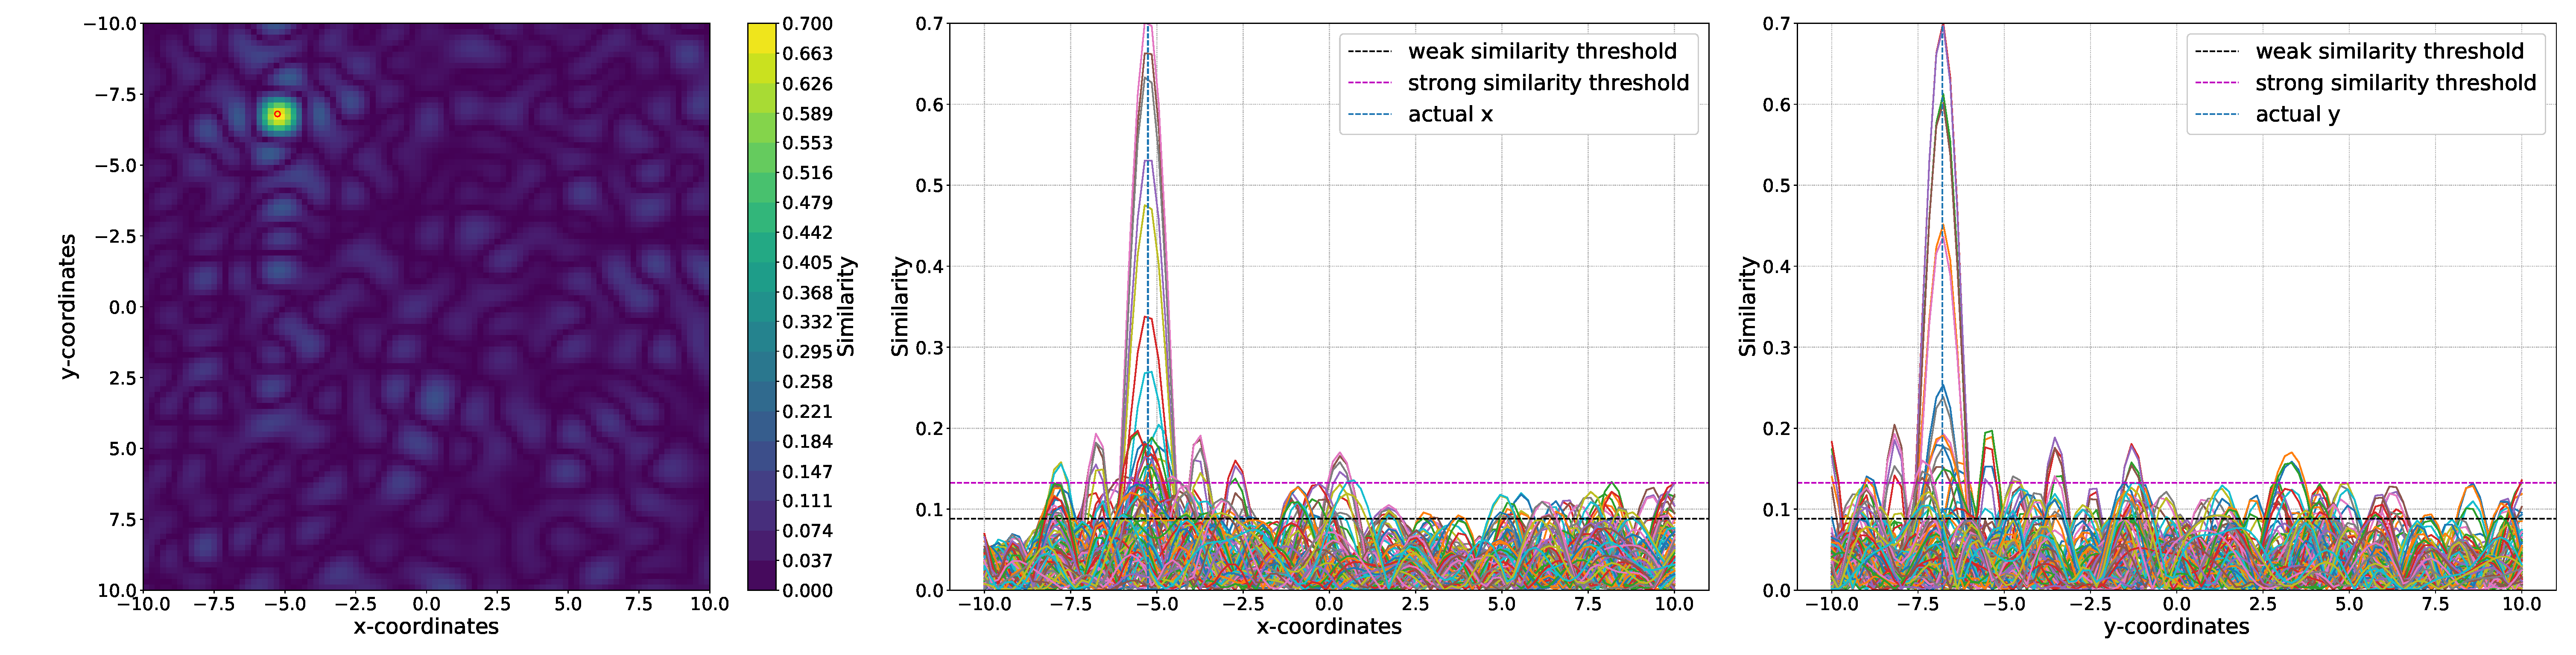
\includegraphics[width=0.9\linewidth]{imgs/spa_power_representation_one_item.eps}
    }\\
    \subfloat[\label{subfig:spa_power_representation_two_items}Convolutive power encoding for two two-dimensional numerical entities]{%
        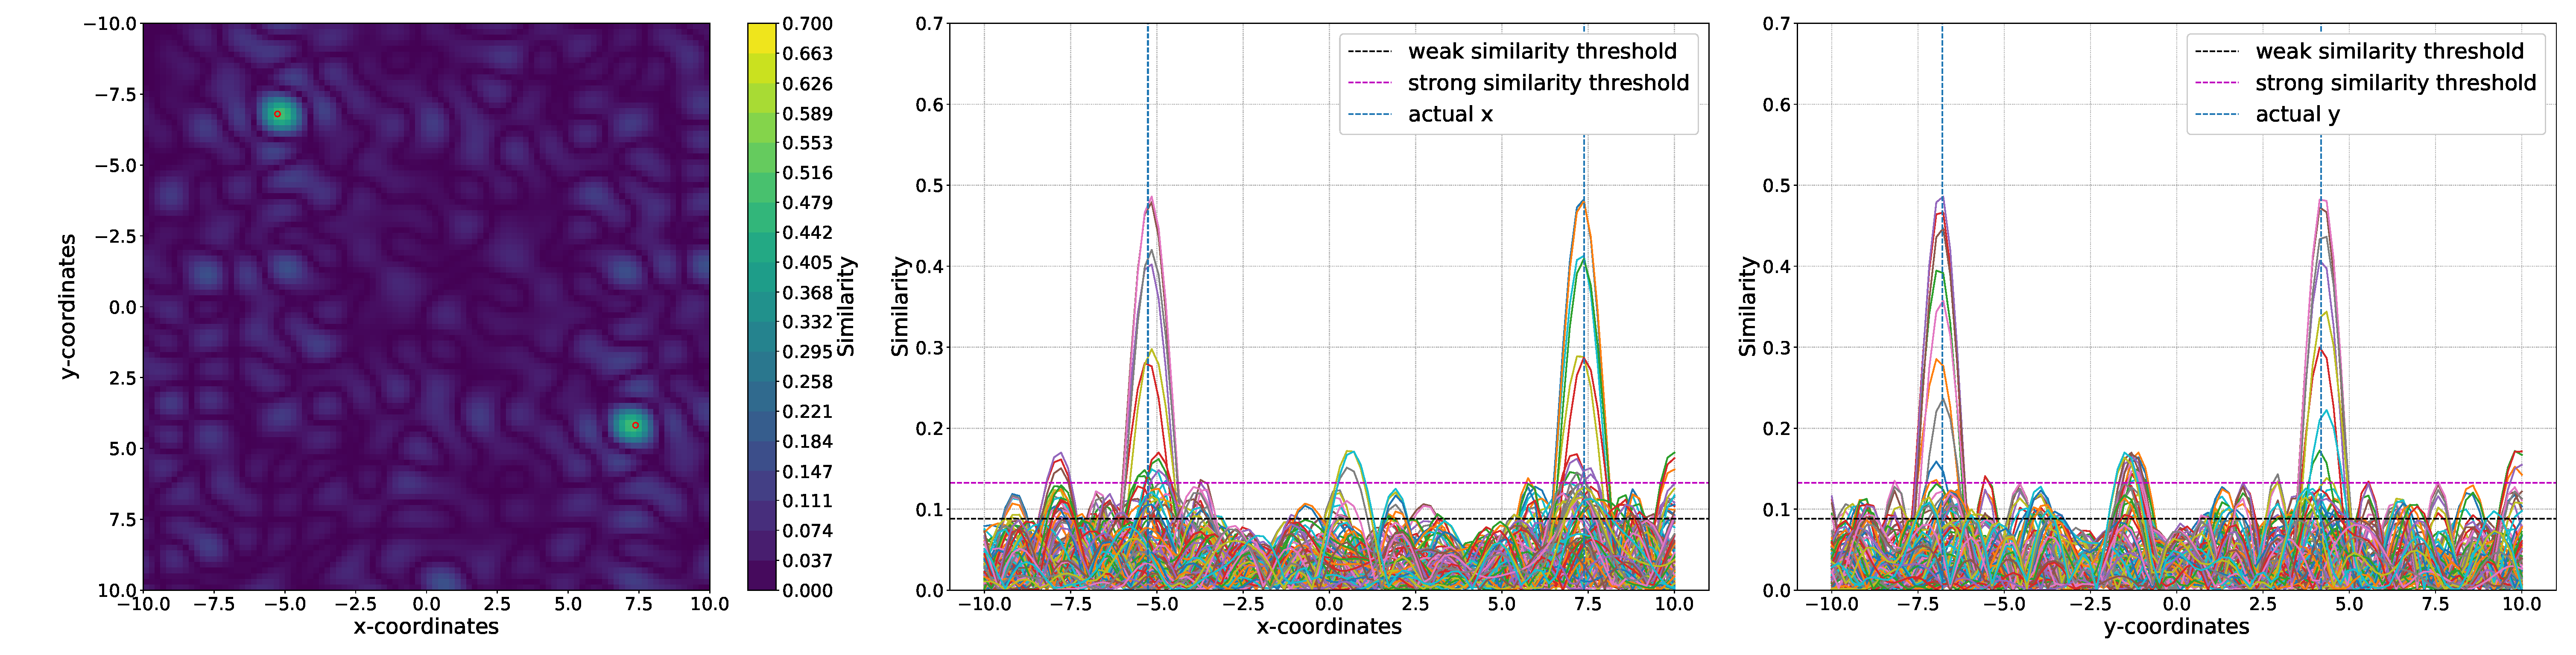
\includegraphics[width=0.9\linewidth]{imgs/spa_power_representation_two_items.eps}
    }
    \caption{
        Visualization of the convolutive power encoding scheme for \num{512}-dimensional representation vectors depicting the similarity between the representation vector and auxiliary comparison vectors created from a sequence of discrete values.
        The left plot in both rows shows a two-dimensional grid of the similarities, while the middle and right plot show the individual entities respectively.
        The red circles in the left plot and the dashed blue lines in the middle and right plots indicate the
    actual encoded values.}
    \label{fig:spa_power_encoding}
\end{figure}

As mentioned previously, we are primarily interested in a way of encoding two-dimensional values in vectors, which is why we focus our analysis of the convolutive power encoding scheme on this case.
Hence, we encode two numerical values $x,y$, i.e., a two-dimensional entity, by generating two random, unitary vectors $ \mathbf{X}, \mathbf{Y} $ representing the corresponding units and applying Equation~\eqref{eq:conv_power_several} 
\begin{equation}
\label{eq:conv_power_2d}
\mathbf{V} = \mathbf{X}^{x} \varoast \mathbf{Y}^{y}.
\end{equation}
To encode a sequence $ \left(x_{i}, y_{i}\right) $ for $i=1, \ldots, n$ of two-dimensional numerical values all sharing the same units, we simply sum up a their individual encoding vectors generated via Equation~\eqref{eq:conv_power_2d}, which leads to
\begin{equation}
\label{eq:conv_power_sum}
\mathbf{V} = \sum\limits_{i=1}^{n} \mathbf{X}^{x_i} \varoast \mathbf{Y}^{y_i}
\end{equation}
Figure~\ref{fig:spa_power_encoding} visualizes vectors encoding one (cf.\ Fig.~\ref{subfig:spa_power_representation_one_item} and Equation~\eqref{eq:conv_power_2d}) and two numerical entities (cf.\ Fig.~\ref{subfig:spa_power_representation_two_items} and Equation~\eqref{eq:conv_power_sum}) given by two units within one vector.
To generate the similarities shown in Fig.~\ref{fig:spa_power_encoding}, we calculate the dot product between the vectors actually representing the encoded values and vectors $ \tilde{\mathbf{V}}_{i} = \mathbf{X}^{\tilde{x}_{i}} \varoast \mathbf{Y}^{\tilde{y}_i} $ encoding a sequence of discrete sample values $ \left( \tilde{x}_{i}, \tilde{y}_{i} \right)$ for $i=1, \ldots, m$.
The left plot in each row of Fig.~\ref{fig:spa_power_encoding} depicts the similarities as heat map over a two-dimensional grid. 
The middle and right plots in Fig.~\ref{fig:spa_power_encoding} visualize the similarities of each unit, which is similar to plotting the heat map in three dimensions as ridges and slicing them through one of the ground axes.
In both rows, we observe high similarity peaks way above both similarity thresholds at the actual encoded values and significantly lower similarity values everywhere else.
However, we already encounter one of the problems of this encoding scheme.
Comparing the similarities at the positions of the encoded values, we observe a drop of similarity values from roughly \num{0.7} to \num{0.5} when encoding two two-dimensional numerical values instead of only one.
Thus, there is a limit of how many values can effectively be encoded in such a representation before noise becomes predominant and the encoded values can not be properly recovered anymore.
Such limitations regarding the number of concepts that can be represented in one vector depending on its dimension are a recurrent theme in the field of \acp{VSA}. 
Furthermore, we picked a $20 \times 20$ grid to encode numerical values using the convolutive power, which shows promising representational features here.
Although we are dealing with real-world sensor measurements in our applications, which are naturally limited by the sensors' range or other physical constraints and/or can be re-scaled to a suitable numerical range, we still need to analyze further, if and why the chosen size of the grid is reasonable.
We will further investigate these limiting factors of our representation in section~\ref{subsec:capacity_analysis_limitations_to_vector_representations}.

\subsection{Structured representations}%
\label{subsec:structured_representations}

Assuming we have generated a suitable vocabulary of atomic vectors encoding the entities and concepts of interest in an automotive context (cf.\ section~\ref{sec:preprocessing_stage_generating_a_vocabulary}) as well as several options of how to encode numerical values in vectors, we are now in the position to encapsulate the content and context of driving situations in semantic vectors.
In general, we employ the \ac{SPA}'s algebraic operations to bind connected items and concepts together through circular convolution and to sum up independent concepts appearing alongside one another.
More particularly, we combine all principles for structured representations presented so far in this thesis: simple superposition to generate unordered sets of items by summing the representational vectors, encoding of bound concepts through role-value pairs as shown in section~\ref{subsec:encoding_struct} and the several approaches to encode numerical values in structured vector representations as shown in section~\ref{subsec:different_vector_representations_for_numerical_values}.
However, the setup of such a vector representation is highly dependent on the actual task to be solved as well as the data available to be encoded.
Thus, we will present and investigate our structured representations in detail for two particular tasks in automotive context, namely driving context classification and vehicle trajectory prediction, in separate chapters~\ref{chap:driving_context_classification} and~\ref{chap:behav_pred}.
However, before we proceed to applying our vector representations to specific automotive tasks, we need to analyze their systematical limitations regarding the amount of information that can effectively be encoded in semantic vectors.

\subsection{Capacity analysis - limiting factors to vector representations}%
\label{subsec:capacity_analysis_limitations_to_vector_representations}

In section~\ref{subsec:different_vector_representations_for_numerical_values} and on several other occasions, we have already seen that there are general and systematical limits for the amount of information that can be encoded in and effectively decoded from vector representations in \acp{VSA}.
Such limits are a reoccurring theme and an essential feature of such architectures as they allow for the modeling of realistic cognitive phenomena.
Considering human subjects for instance, the capacity to process and store information or concepts in short-term memory as well as other cognitive tasks is subject to numerical restrictions \parencite{Miller1956}.
Hence, numerical limitations of cognitive architectures like the \ac{SPA} or \acp{VSA} in general are one way of modeling the numerical restrictions to cognition observed in human subjects.
In the context of automated driving however, we need to analyze these restrictions imposed by the cognitive architecture applied to provide upper borders regarding the amount of information that can be stored in our vector representation.
In this section, we analyze these limits with the goal of finding bounds for, e.g., the number of concepts that can effectively be stored in a single vector before the accumulation of noise makes it impossible to retrieve the original individual vectors.

\subsubsection{Superposition capacity}%
\label{ssubsec:superposition_capacity}

\begin{figure}[t]
	\centering
	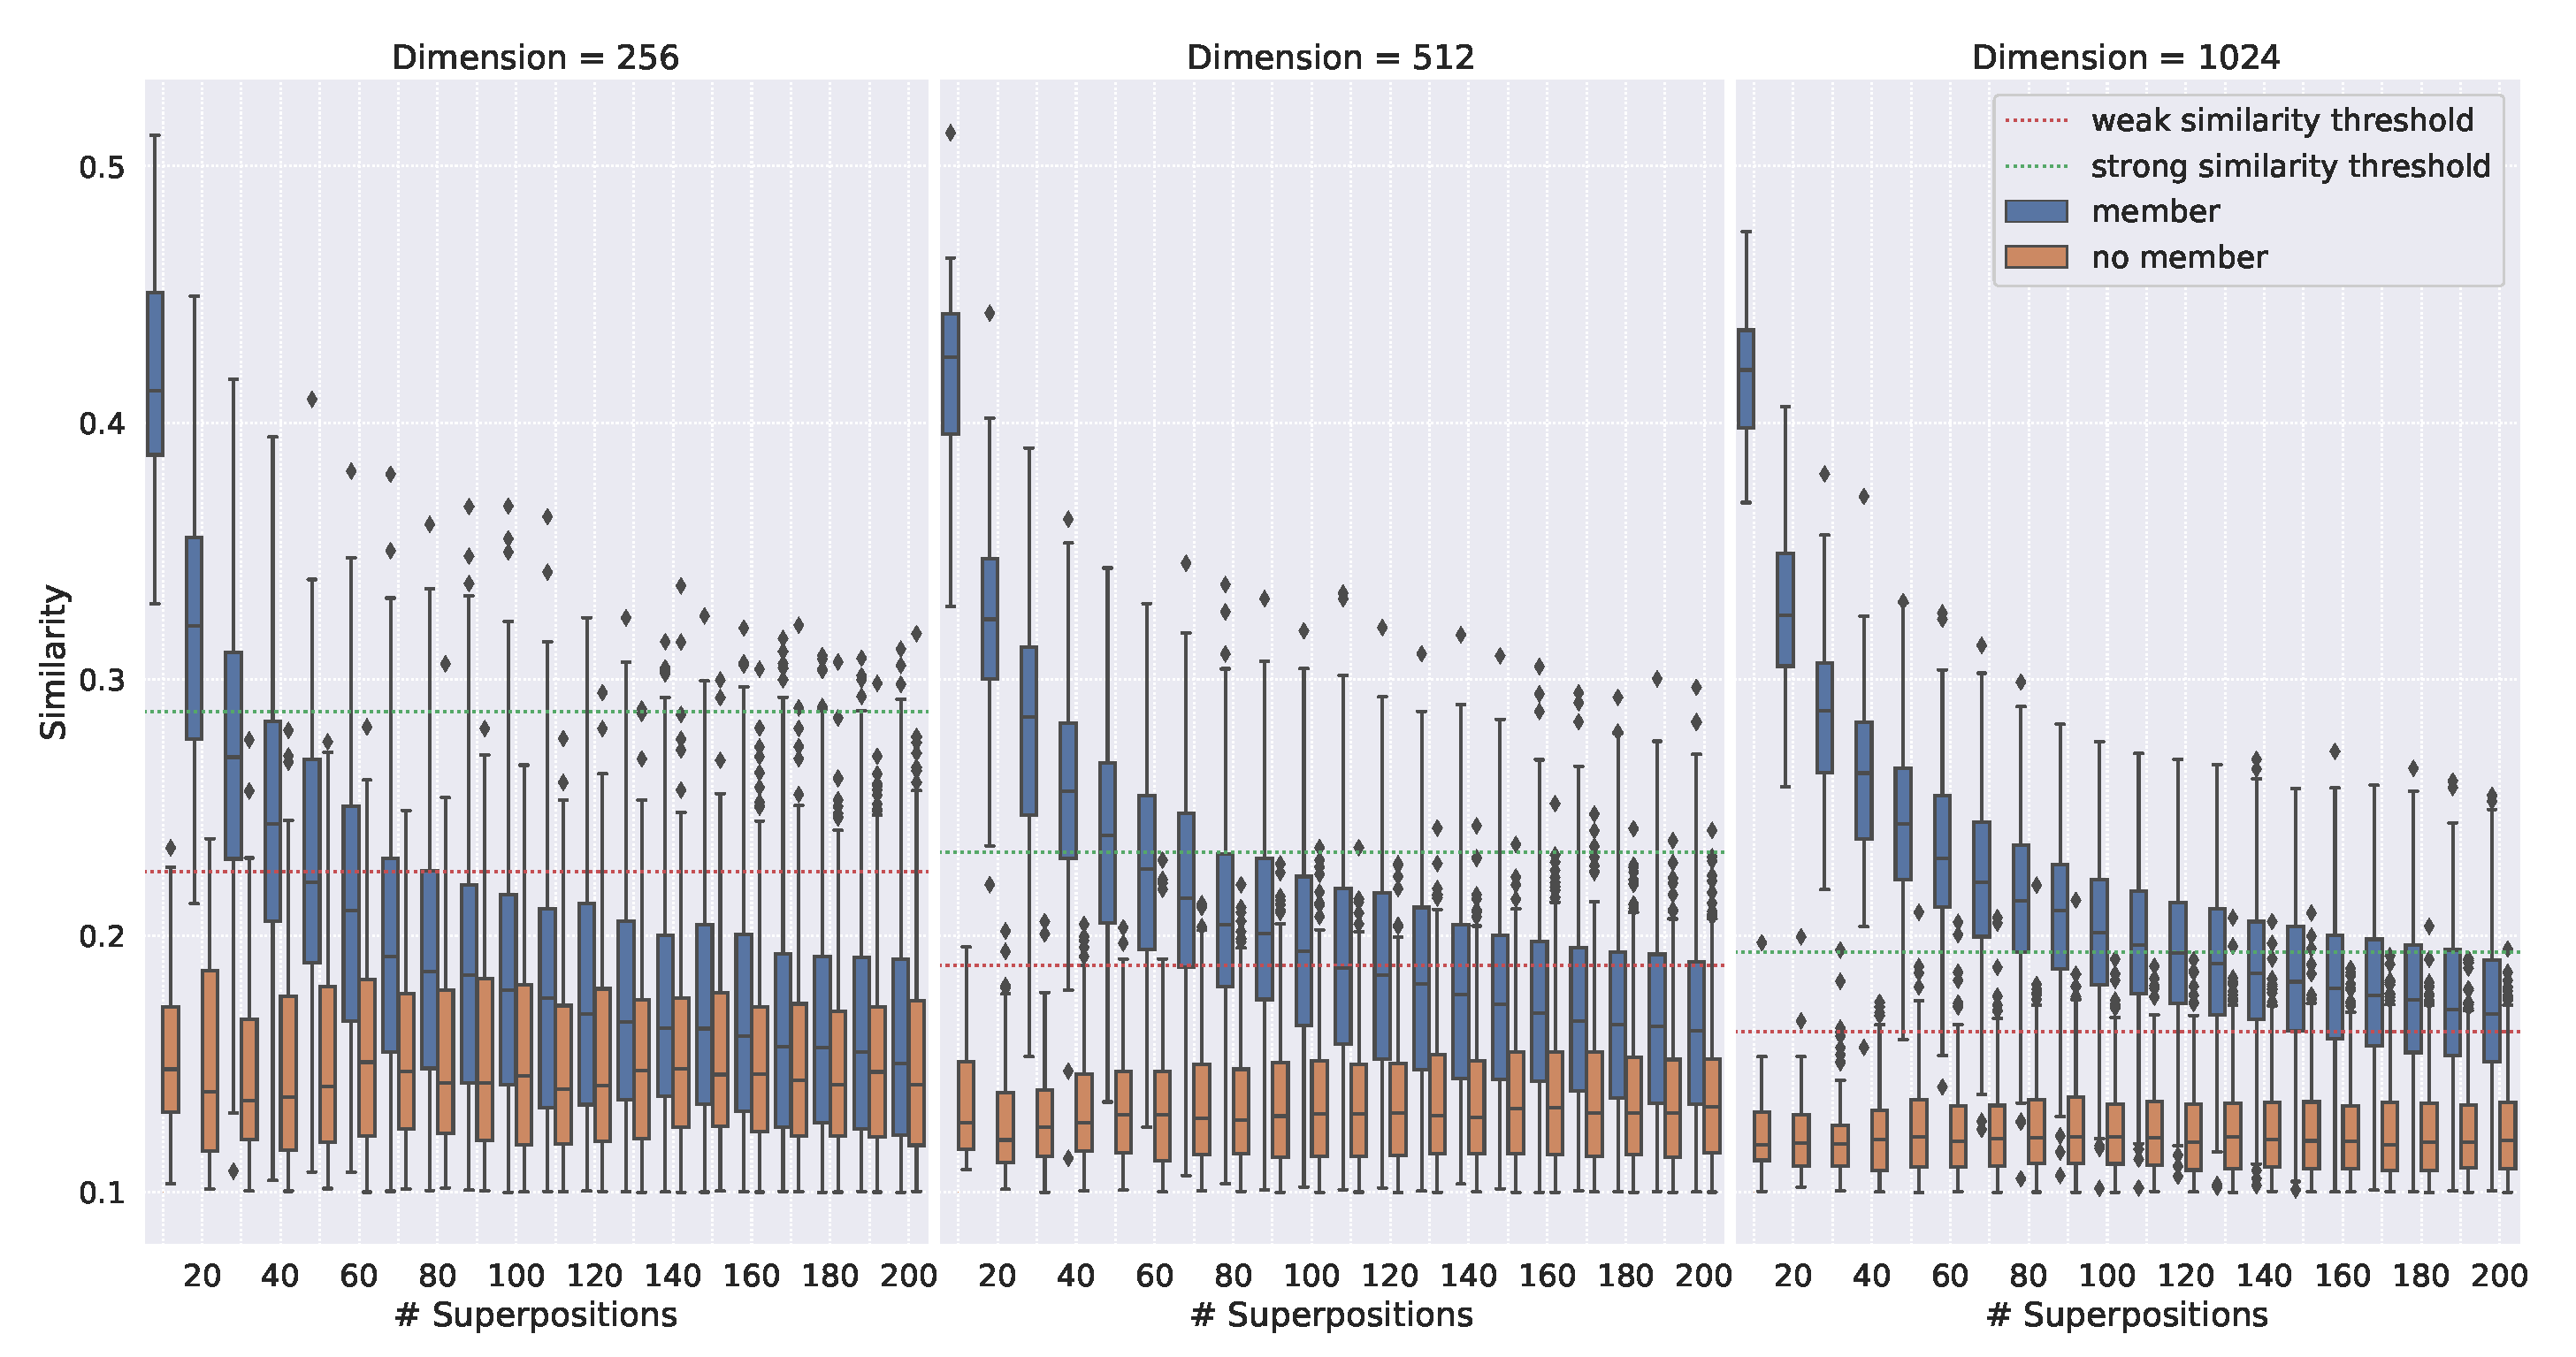
\includegraphics[width=0.95\textwidth]{imgs/spa_superposition_capacity.eps}
	\caption{Visualization of the \ac{SPA}'s superposition capacity for vector dimensions \num{256}, \num{512} and \num{1024}.
    The blue boxes indicate the similarity between the superposition vector and its summands, the orange boxes illustrate the similarity between the superposition vector and other randomly generated vectors.
    The dotted lines visualize the similarity threshold based on the vector dimensionality for reference.}
	\label{fig:spa_superposition_capacity}
\end{figure}

First, we evaluate the capacity of superposition, i.e., the addition operation of the \ac{SPA}.
Superposition is used to store and combine several concept vectors $ \mathbf{v}_i$ for $i=0, \ldots, n$ in an unordered set
\begin{equation}
\label{eq:superposition}
\mathbf{s} = \sum\limits_{i=0}^{n} \mathbf{v}_{i}.
\end{equation}
Given the properties of the \ac{SPA}, we can determine if a vector of interest $\mathbf{w}$ belongs to that ordered set by calculating the similarity $\phi\left( \mathbf{s}, \mathbf{w}\right)$ between the superposition vector and the vector of interest.
For sufficiently high-dimensional vectors, the similarity $\phi\left( \mathbf{s}, \mathbf{w}\right)$ will be close to \num{0} in case the vector $ \mathbf{w}$ is not part of the sum.
However, the more vectors we add to the superposition vector $ \mathbf{s}$, the more noise accumulates in the representation and thus decreases the similarity between the superposition vector $ \mathbf{s}$ and its individual ingredients $ \mathbf{v}_i$.
In order to analyze how many vectors can be added together by superposition before individual vectors become irretrievable, we conducted the following experiment: assuming we want to add $n$ vectors $ \mathbf{v}_i$ for $i=1, \ldots, n$ into a superposition vector $ \mathbf{s}$ as in Equation~\eqref{eq:superposition}, we randomly generate a vocabulary of $2n$ vectors $ \mathbf{v}_i$ for $i=1, \ldots, 2n$ and sum up the first $n$ members to create our superposition vector $ \mathbf{s}$.
Then we calculate the cosine similarity $\phi\left(\mathbf{s}, \mathbf{v}_i\right)$ between the superposition vector $ \mathbf{s}$ and every vector $ \mathbf{v}_{i}$ for $i=1,\ldots, 2n$ in the vocabulary.
A similar but slightly different experiment has been conducted by \textcite{Wahle2012}: the atomic vocabulary vectors,  referred to as elemental vectors in \textcite{Wahle2012}, are sparse in the sense, that they mostly contain \num{0} elements, and the superposed vectors are normalized after adding them.
Furthermore, \textcite{Wahle2012} only compare the similarity $\phi\left(\mathbf{s}, \mathbf{v}_1\right)$ between the superposition and the original vector with the similarity $\phi\left(\mathbf{v}_1, \mathbf{v}_n\right)$ between the original vector $ \mathbf{v}_1$ and the most recently added random vector $ \mathbf{v}_{n}$ as baseline for the expected similarity between randomly chosen vectors.
In contrast, although we have already analytically derived a threshold $\epsilon= \tfrac{c}{\sqrt{D}}$ for the expected similarity of randomly chosen vectors in definition~\ref{def:similar}, we calculate the similarity between the superposition vector and $n$ other random vectors for reference.

Figure~\ref{fig:spa_superposition_capacity} shows the result of our experiment for \num{3} random vocabularies per superposition length containing vectors of dimension \num{256}, \num{512} and \num{1024}.
The blue boxes in each figure illustrate the similarity between the superposition vector $ \mathbf{s}$ and each of the individual vectors $ \mathbf{v}_i$ for $i=1, \ldots, n$ it contains, i.e., the members of the unordered superposition set.
The orange boxes depict the similarity between $ \mathbf{s}$ and the other vocabulary vectors $ \mathbf{v}_i$ for $i=n+1, \ldots, 2n$ it does not contain, i.e., the non-members.
The dotted red and green lines indicate the \ac{SPA}'s weak and strong similarity threshold depending on the dimension of the vector space.
Considering the weak similarity threshold $\epsilon_{weak} = \tfrac{2}{\sqrt{D}}$, we observe that for a vector dimension of \num{256} the \ac{SPA} allows roughly \num{50} items to be stored in a superposition vector.
For higher vector dimensions \num{512} and \num{1024}, the number of items that can be superposed increases to roughly \num{100} and \num{200} respectively.
Considering the strong similarity threshold $\epsilon_{strong} = \tfrac{3}{\sqrt{D}}$, the upper borders for the number of items being stored in a superposition vector are slightly more conservative with \num{25}, \num{50} and \num{100} for vector space dimensions of \num{256}, \num{512} and \num{1024} respectively.
We also observe in our experiments that the similarity between the superposition vector and non-member random vectors is consistently below the weak similarity threshold $\epsilon_{weak}$ for the majority of the samples.
However, once the similarity between the superposition vector and its members drops below either of the similarity thresholds for the majority of the samples, we can not distinguish between members and non-members with a sufficiently high probability.
For \num{256} dimensional vectors for instance, we even observe that the members and non-members become nearly indistinguishably when adding more than \num{80} vectors.
Thus, we have to choose rather conservative bounds for the number of items to be encoded in a superposition vector.

\subsubsection{Capacity of structured representations involving convolutive powers}%
\label{ssubsec:capacity_of_structured_representations_involving_convolutive_powers}

\begin{figure}[t]
    \centering
    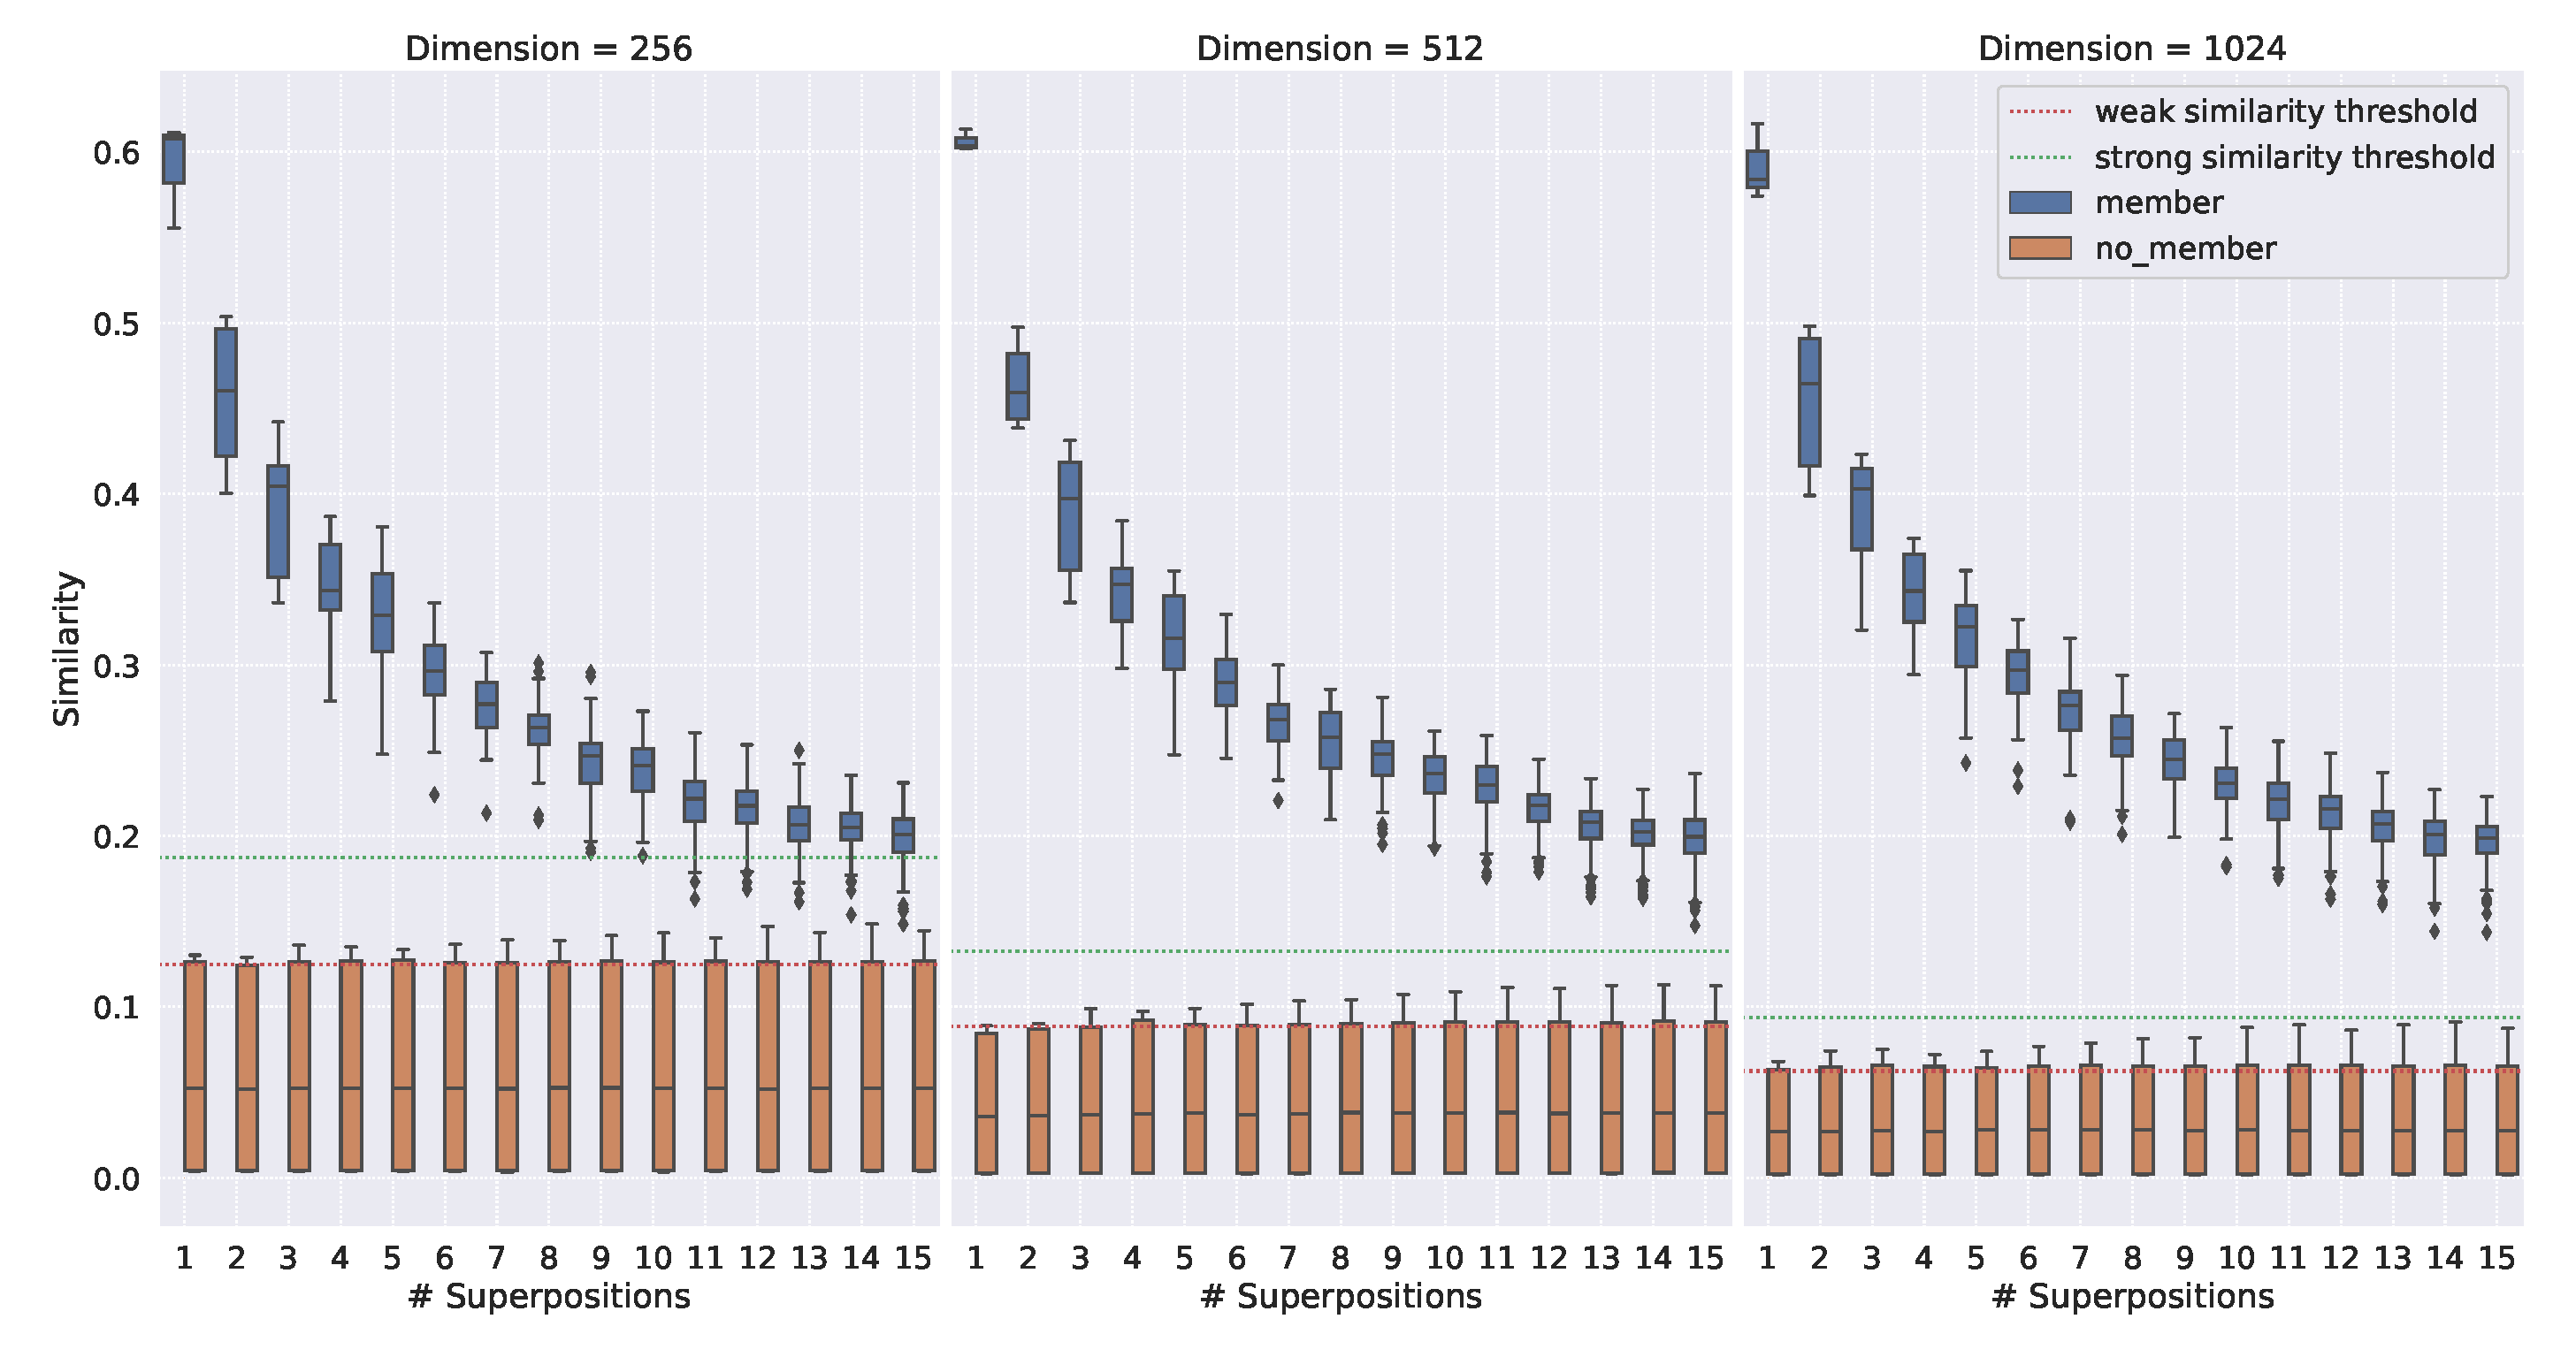
\includegraphics[width=0.95\linewidth]{imgs/spa_power_capacity.eps}
    \caption{Capacity analysis for the superposition of vectors encoding spatial positions using the convolutive vector-power for varying vector dimensions.}
    \label{fig:spa_power_capacity}
\end{figure}

In the previous section, we have analyzed the \ac{SPA}'s capacity regarding the number of items that can be stored in an unordered set using superposition.
For encoding driving situations in a semantic vector substrate, we will most likely employ more complex representation than superposition of single items alone.
In this section, we thus analyze the \ac{SPA}'s capacity regarding the structured representations involving the convolutive vector-power representation presented in section~\ref{subsec:different_vector_representations_for_numerical_values}.
Figure~\ref{fig:spa_power_encoding} has already shown, that unbinding positions back out by querying the representation vector with sample vectors encoding discrete position examples yields high similarities for samples in the region of the encoded values and low similarities elsewhere.
These low similarities for the particular examples shown in Fig.~\ref{subfig:spa_power_representation_one_item} and~\ref{subfig:spa_power_representation_two_items} are below or at most in the order of magnitude of the \ac{SPA}'s similarity thresholds.
However, we also observe, that encoding several entities of the same type in one position vector as in Fig.~\ref{subfig:spa_power_representation_two_items}, the similarities of the true positive positions decrease compared to the encoding of only one item as in Fig.~\ref{subfig:spa_power_representation_one_item}.
Hence, our capacity analysis not only has to cover the amount of objects encoded in one vector, but also the number of items per object class.

\begin{figure}[t]
    \centering
    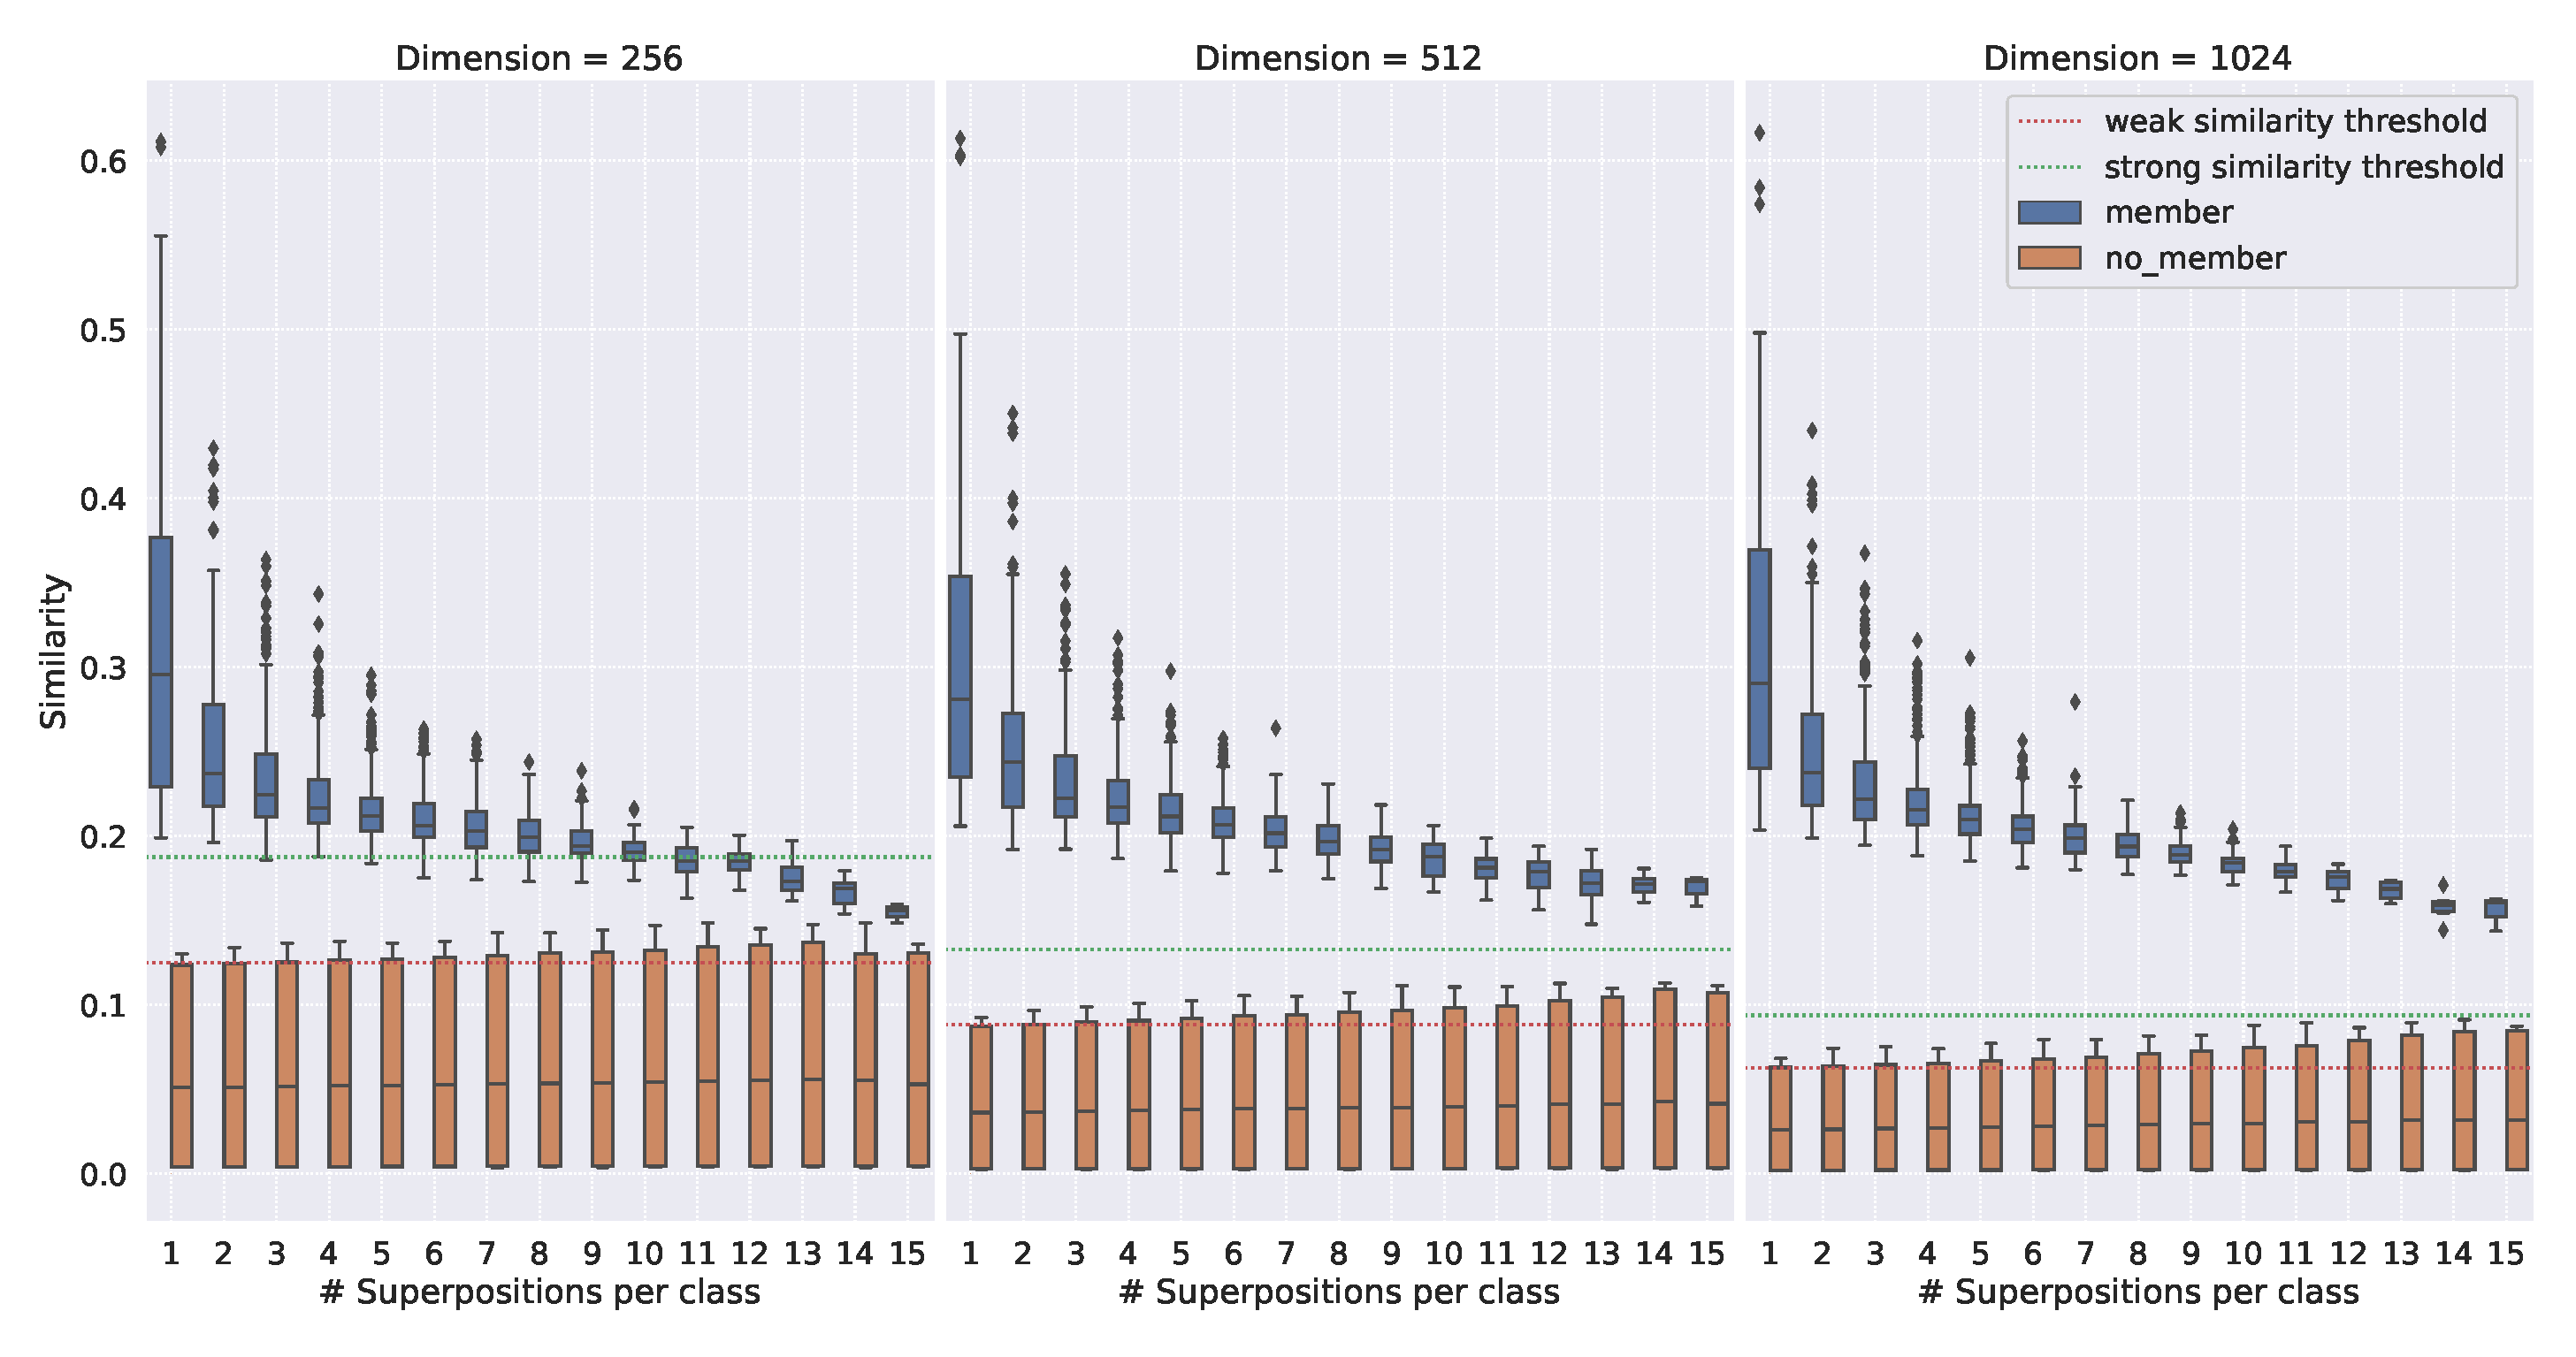
\includegraphics[width=0.95\linewidth]{imgs/spa_power_capacity_superpositions_per_class.eps}
    \caption{Capacity analysis for the superposition of vectors encoding spatial positions using the convolutive vector-power for varying vector dimensions.
        In contrast to Fig.~\ref{fig:spa_power_capacity}, this figure illustrates the similarity for vectors containing spatial information for several objects of the same class.
    }
    \label{fig:spa_power_capacity_superpositions_per_class}
\end{figure}

Therefore, we conduct the following experiment: assuming we want to encode $n$ spatial entities, i.e., objects $o_{i}$ with two-dimensional location information $ \left(x_{i}, y_{i}\right)$ for $i=1, \ldots, n$ as shown in Fig.~\ref{fig:spa_power_encoding} for $n=1$ (Fig.~\ref{subfig:spa_power_representation_one_item}) and $n=2$ (Fig.~\ref{subfig:spa_power_representation_two_items}), into a single representation vector $ \mathbf{s}$, we generate a vocabulary of random vectors $
\mathbf{v}_{i}$ for $i=1, \ldots, n$ encoding object class labels and random unitary vectors $ \mathbf{X}, \mathbf{Y}$ to encode the units of the spatial information.
In contrast to the previous experiment, where we simply summed up a certain number of random vectors, we are interest in a more specific analysis, since there are several possibilities to distribute the positional values $ \left(x_{i}, y_{i}\right)$ over the available object class vectors $ \mathbf{v}_{i}$.
For instance, for a total number of two superpositions, i.e., $n=2$, there are two possibilities to generate our representation vector, namely
\begin{align}
    \mathbf{s}_{1} &= \mathbf{v}_{1} \varoast \mathbf{X}^{x_{1}} \varoast \mathbf{Y}^{y_{1}} + \mathbf{v}_{1} \varoast \mathbf{X}^{x_{2}} \varoast \mathbf{Y}^{y_{2}}, \label{eq:spa_power_exp_v1} \\
    \mathbf{s}_{2} &= \mathbf{v}_{1} \varoast \mathbf{X}^{x_{1}} \varoast \mathbf{Y}^{y_{1}} + \mathbf{v}_{2} \varoast \mathbf{X}^{x_{2}} \varoast \mathbf{Y}^{y_{2}}. \label{eq:spa_power_exp_v2} 
\end{align}
The vector $ \mathbf{s}_{1}$ in Equation~\eqref{eq:spa_power_exp_v1} encodes two objects of the same type, while the vector $ \mathbf{s}_{2}$ encodes occurrences of two different object types at the given locations.
As we are working with random vectors in this experiment, we can, without loss of generality, skip the vector encoding two objects of type represented by the vector $ \mathbf{v}_{2}$, which would yield a result equivalent to Equation~\eqref{eq:spa_power_exp_v1}.
More generally, we are interested in all sets
\begin{equation}
\label{eq:sum_combinations}
C_{m,j} = \left\{0 < k_{1}, \ldots, k_{m} \leq n \quad | \quad m \leq n \textrm{ and } \sum\limits_{i=1}^{m} k_{i} = n \right\}
\end{equation}
of natural numbers $k_{i}$ summing up to $n$ ignoring permutations of the $k_{i}$. 
We index the sets with $j$, since there potentially exist several possibilities to decompose $n$ into sums of $m$ natural numbers.

In our experiments, for each number $n$ of total objects to be encoded in the vector representation, we calculate all possible sets $C_{m,j}$ (ignoring permutations) and generate random position values $ \left(x_{i}, y_{i}\right)$ for $i=1, \ldots, n$ and a random vocabulary as described above.
For each set $C_{m,j}$, we generate a representation vector 
\begin{equation}
\label{eq:spa_power_exp_v_gen}
\mathbf{s}_{m,j} = \sum\limits_{i=1}^{m} \sum\limits_{l=1}^{k_{i}} \mathbf{v}_{i} \varoast \mathbf{X}^{x_{i}} \varoast \mathbf{Y}^{y_{i}}
\end{equation}
as well as query vectors $ {\mathbf{P}}_{i} = \mathbf{X}^{\tilde{x}_{i}} \varoast \mathbf{Y}^{\tilde{y}_i} $ encoding a sequence of discrete sample values $ \left( \tilde{x}_{i}, \tilde{y}_{i} \right)$ for $i=1, \ldots, M$ evenly distributed over the length of the positional encoding grid.
In other words, Equation~\eqref{eq:spa_power_exp_v_gen} states, that each class label $ \mathbf{v}_{i}$ appears $k_{i}$ times yielding a sum of $n$ objects.
We query the representation vector for the position of each class by binding it to the pseudo-inverse element $ \bar{ \mathbf{v}}_{i}$ for each class label vector, i.e., 
\begin{equation}
\label{eq:spa_power_query}
\mathbf{s}_{m,j} \varoast \bar{ \mathbf{v}}_{i} \approx \sum\limits_{l=1}^{k_{i}} \mathbf{X}^{{x}_{i}} \varoast \mathbf{Y}^{{y}_i}, 
\end{equation}
and calculate the similarity with the discretized position vectors $ \mathbf{P}_{k}$ to get
\begin{equation}
\label{eq:text}
s_{i,k} = \left|\phi \left( \mathbf{s}_{m,j} \varoast \bar{ \mathbf{v}}_{i}, \mathbf{P}_{k}\right) \right|.
\end{equation}
For samples close to the originally encoded positions, i.e., $\left| x_{i} - \tilde{x}_{i}\right| < \epsilon$ and $\left| y_{i} - \tilde{y}_{i}\right| < \epsilon$ for a certain threshold $\epsilon$, we label $s_{i,k}$ as positive similarity denoting a member of the representation vector.
Otherwise, we consider the similarity $s_{i,k}$ at position $\left( \tilde{x}_{i}, \tilde{y}_{i} \right)$ not a member of the representation vector $ \mathbf{s}_{m,j}$.

Figure~\ref{fig:spa_power_capacity} shows the results of this capacity analysis regarding the total number of superposed objects within the representation vector for varying vector dimensions.
The blue boxes in each column illustrate the positive similarity values, i.e., for positions considered members of the representation vector, whereas the orange boxes indicate the negative similarity values of the non-member positions.
The dotted red and green lines visualize the weak and strong similarity threshold for each dimension respectively.
Similar to Fig.~\ref{fig:spa_power_encoding}, we observe that the similarity of the non-members is in the order of magnitude of the similarity thresholds while the similarity for the member position decreases with a growing number of spatial items encoded in the vector.

Figure~\ref{fig:spa_power_capacity_superpositions_per_class} shows a different evaluation of the same data showing the number of addition operations per class on the $x$-axis.
In contrast to Fig.~\ref{fig:spa_power_capacity}, Fig.~\ref{fig:spa_power_capacity_superpositions_per_class} illustrates the similarity for vectors containing spatial information for several objects of the same class.
That is, Fig.~\ref{fig:spa_power_capacity_superpositions_per_class} illustrates the similarity of vectors containing a specific number $n$ of superpositions per class on its $x$-axis independent of the total number of superpositions.
We observe, that not only the similarity of the members decreases with growing number of superpositions per class, but the similarity of the non-member increases beyond the weak similarity threshold.
Similar to the simple superposition capacity analysis, we consider the point in the plots where the member similarities fall below the strong similarity threshold the upper border for the maximal number of spatial objects per class to be encoded in this representational substrate.
For instance, this upper bound for \num{256} dimensional vectors is \num{10} superpositions per class, which is roughly half of the upper bound for the number of simple superpositions.

\section{Summary}%
\label{sec:vector_representations_automotive_summary}

In this chapter, we presented the general approach of creating structured vector representations to encode automotive scenes.
After showing the theoretical tool set in chapter~\ref{chap:introduction_to_vsas} independent of particular applications, we focused our attention to scene representation in automotive context.
The chapter's structure followed the process established by \textcite{Gallant2013} and is split into two main subsections focusing on the creation of vocabularies of atomic vectors (section~\ref{sec:preprocessing_stage_generating_a_vocabulary}) and generating structured, more complex representations from the atomic vectors in the vocabulary (section~\ref{sec:representation_generation_stage}).
We showed several approaches to generate vector vocabularies of entities encountered in automotive scenes such as traffic participants and traffic signs based on either manual design or automated learning.
Thereby, we were able to encapsulate different similarity structures such as visual similarity, semantic similarity and a fusion of both.
We were able to demonstrate, that we can successfully encapsulate the desired similarity structure within our vocabulary of atomic vectors.
Finally, we pointed out advantages and problems for both approaches to generate these structured vocabularies with the bias imposed by human engineers and limits regarding sufficiently large and available data sets being the main issues for manual and learned vocabularies respectively.
Since we consider the choice of a suitable vocabulary to be highly dependent on the particular task to be solved, we analyze the influence of varying the underlying vocabulary for the specific task of classifying the current driving context based on a vector representation of the current scene in section~\ref{subsec:the_influence_of_varying_vocabularies}.

In section~\ref{sec:representation_generation_stage}, we proceeded to investigate the creation of more complex, structured representations from atomic vocabulary vectors.
One of the most important aspects was the representation of numerical values in high-dimensional vectors, where we presented three different approaches and showed their individual strengths and limitations.
Particularly, we presented a novel approach to encode numerical values based the convolutive power of vectors.
The biggest advantage of this representation of numerical values is that it can be bound further to other vectors as well as be used to query representation vectors about location information using pseudo-inverse elements.
This approach is the main building block of the scene representation used as input to the learning models for vehicle trajectory prediction proposed in chapter~\ref{chap:behav_pred}.
Finally, we analyzed the capacity of structured vector representations based on simple superposition and superposition combined with the convolutive power encoding of spatial information.
Thereby, we found upper bounds for the amount of information that can effectively be encoded in such representations.
These bounds have to considered in subsequent chapters to evaluate if the amount of information to be encoded in the vector representation is compliant with the bounds.
This will allow a conclusive assessment of the limits of structured vector representations in automotive context.
In the next chapter, we now turn our focus towards a concrete application scenario, namely the classification of the current driving context based on a structured vector representation of the current scene.

